%%%%%%%%%%%%%%%%%%%%%%%%%%%%%%% beamer %%%%%%%%%%%%%%%%%%%%%%%%%%%%%%%%%%%%%%%%%%%%%%%%%
%%%%%%%%%%%%%%%%%%%%%%%%%%%%%%% beamer %%%%%%%%%%%%%%%%%%%%%%%%%%%%%%%%%%%%%%%%%%%%%%%%%
% To run - pdflatex filename.tex
%	   acroread filename.pdf
%%%%%%%%%%%%%%%%%%%%%%%%%%%%%%%%%%%%%%%%%%%%%%%%%%%%%%%%%%%%%%%%%%%%%%%%%%%%%%%%%%%%%%%%
%\documentclass[handout,compress,green]{beamer}
\RequirePackage{flashmovie}
\documentclass[compress,pink]{beamer}
\usetheme{boxes}
%\hypersetup{pdfpagemode=FullScreen}%makes your presentation go automatically to full screen
\usepackage[absolute,overlay]{textpos}
\setlength{\TPHorizModule}{1mm}
\setlength{\TPVertModule}{1mm}

\useoutertheme[subsection=false]{smoothbars}
\beamertemplateshadingbackground{white!25}{pink!10}
\setbeamertemplate{footline}[text line]{} % makes the footer EMPTY

% include packages
\usepackage{subfigure}
%\usepackage{natbib}
%\usepackage{biblatex}
\usepackage{multicol}
\usepackage{epsfig}
\usepackage{graphicx}
\usepackage{amssymb,amsmath}
\usepackage[all,knot]{xy}
\xyoption{arc}
\usepackage{url}
\usepackage{multimedia}
\usepackage{hyperref}
\usepackage[utf8]{inputenc}
%\usepackage[utf8]{fontenc}
\usepackage{lmodern}
\usepackage[swedish]{babel}
\usefonttheme{professionalfonts}
\usepackage{times}
\usepackage{tikz}
\usepackage{amsmath}
\usepackage{amsthm}
\usepackage{verbatim}
\usepackage{multirow}
\usepackage{blindtext}
\usepackage{biblatex}

\usetikzlibrary{arrows,shapes} 
%%%%%%%%%%%%%%%%%%%%%%%%%%%%%%%%%%%%%%%%%%%%%%%%%%%%%%%%%%%%%%%%%%%%%%%%%%%%%%%%%%%%%%%%%%
%%%%%%%%%%%%%%%%%%%%%%%%%%%%%% Title Page Info %%%%%%%%%%%%%%%%%%%%%%%%%%%%%%%%%%%%%%%%%%%
%%%%%%%%%%%%%%%%%%%%%%%%%%%%%%%%%%%%%%%%%%%%%%%%%%%%%%%%%%%%%%%%%%%%%%%%%%%%%%%%%%%%%%%%%%
\bibliography{MelianUZurichMAR2019.bib}

\vspace{-8 in}
\title{}\\

\vspace{0.4 in}
\tiny Carlos J. Meli\'an\\ETH-EAWAG\\
https://github.com/melian009
\vspace{4.5 in}
\pgfdeclareimage[width=9cm]{mybackground}{evo1v2.pdf}
\setbeamertemplate{title page}{

        \begin{picture}(2,2)
\vspace{1.5 in}
            \put(130,-60){%
                \pgfuseimage{mybackground}
            }
            \put(0,-110.7){%
                \begin{minipage}[b][45mm][t]{26mm}
                    \usebeamerfont{title}{\inserttitle\par}
                \end{minipage}
            }
            \end{picture}
    }
\vspace{-1.5 in}
\date{}

%%%%%%%%%%%%%%%%%%%%%%%%%%%%%%%%%%%%%%%%%%%%%%%%%%%%%%%%%%%%%%%%%%%%%%%%%%%%%%%%%%%%%%%%%%
%%%%%%%%%%%%%%%%%%%%%%%%%%%%%% Begin Your Document %%%%%%%%%%%%%%%%%%%%%%%%%%%%%%%%%%%%%%%
%%%%%%%%%%%%%%%%%%%%%%%%%%%%%%%%%%%%%%%%%%%%%%%%%%%%%%%%%%%%%%%%%%%%%%%%%%%%%%%%%%%%%%%%%%
\begin{document}
\vspace{-2 in}
\hspace{-0.04 in}{\Large \textcolor{black}{Eco-}\textcolor{red}{Evolutionary} \textcolor{blue}{Networks}}
	\titlepage
\vspace{0.1 in} {\tiny \textcolor{blue}{U. Z\"urich, 28 March 2019 -- Ecological Networks BIO365}}
\newpage

\section{Motivation}

%==========NOTES TALKS============================================================================================================
%Gain intuition about biodiversity and eco evo feedbacks
%=================================================================================================================================


%Global map biodiversity gradient + biodiversity loss : causes? (3 slides)
\subsection{Latitudinal biodiversity gradient}
\frame{\frametitle{{\small}}
  \begin{center}
    \vspace{-0.25 in}
  \hspace{-0.25 in}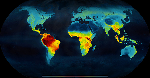
\includegraphics[height=7cm,width=11cm]{Figure1Mannion.pdf}
\end{center}
}

\subsection{Heterogeneous biodiversity loss}
\frame{\frametitle{{\small}}
  \begin{center}
    \vspace{-0.25 in}
  \hspace{-0.25 in}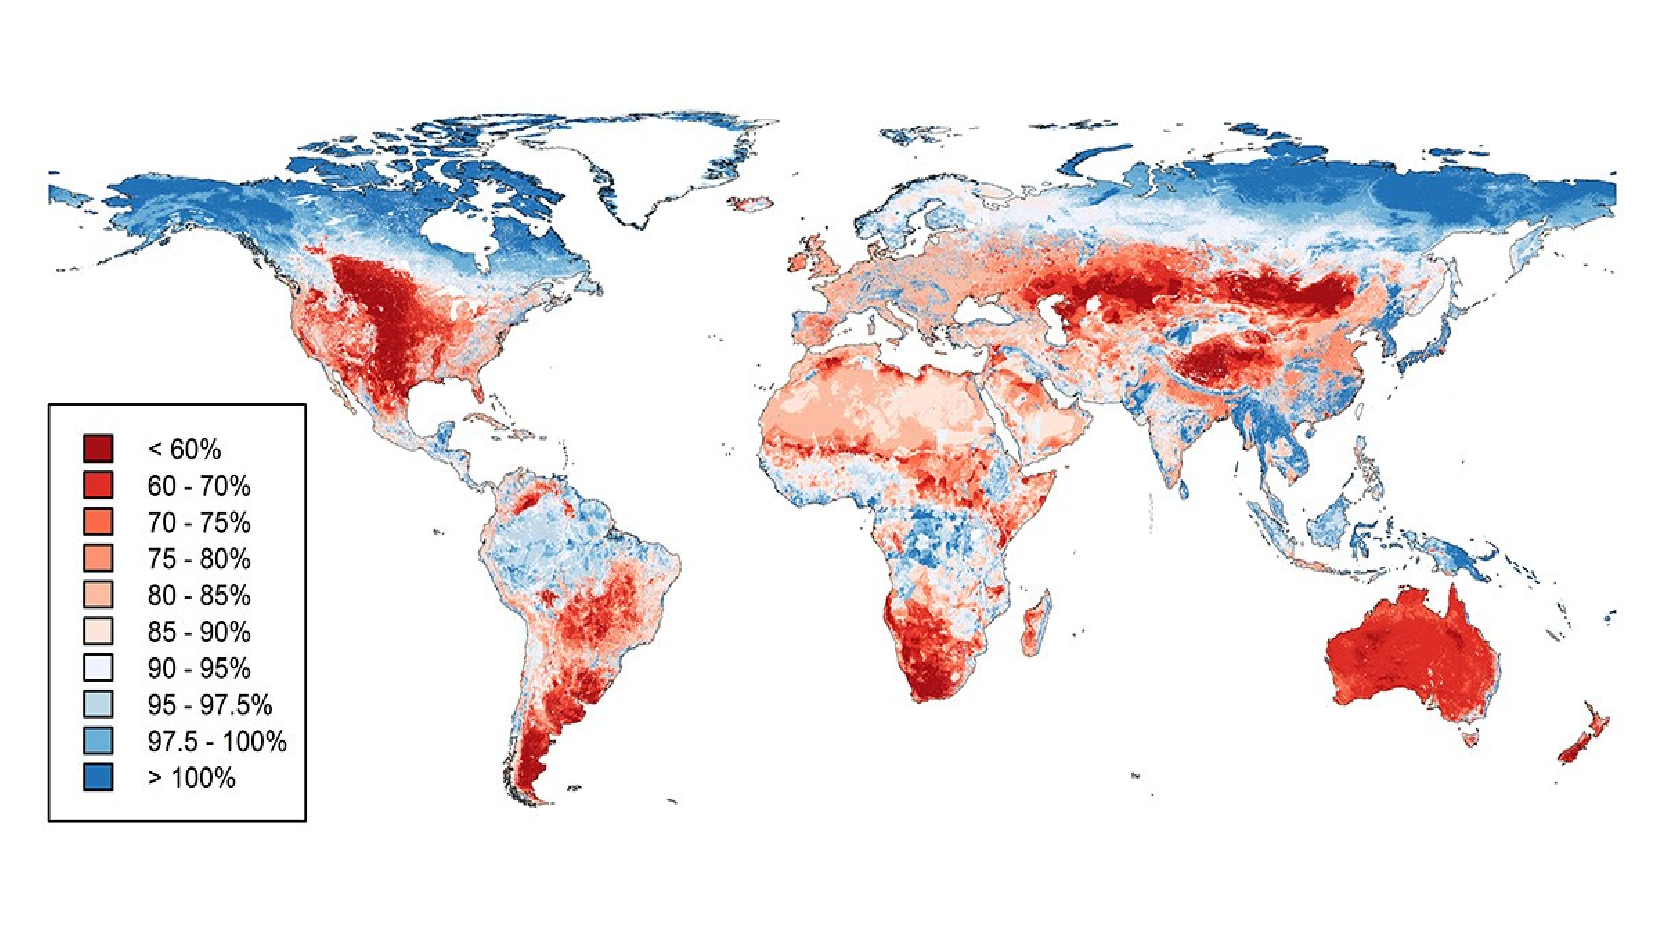
\includegraphics[height=7cm,width=11cm]{BiodiversityLoss.pdf}
\end{center}
}

\subsection{Architecture of ecosystems}
\frame{\frametitle{{\small}}
  \setbeamercolor{uppercol}{fg=black,bg=white}
  \setbeamercolor{lowercol}{fg=black,bg=white}
  \begin{beamerboxesrounded}[upper=upperco,lower=lowercol,shadow=true]{}
\begin{center}
  \hspace{-0.45 in}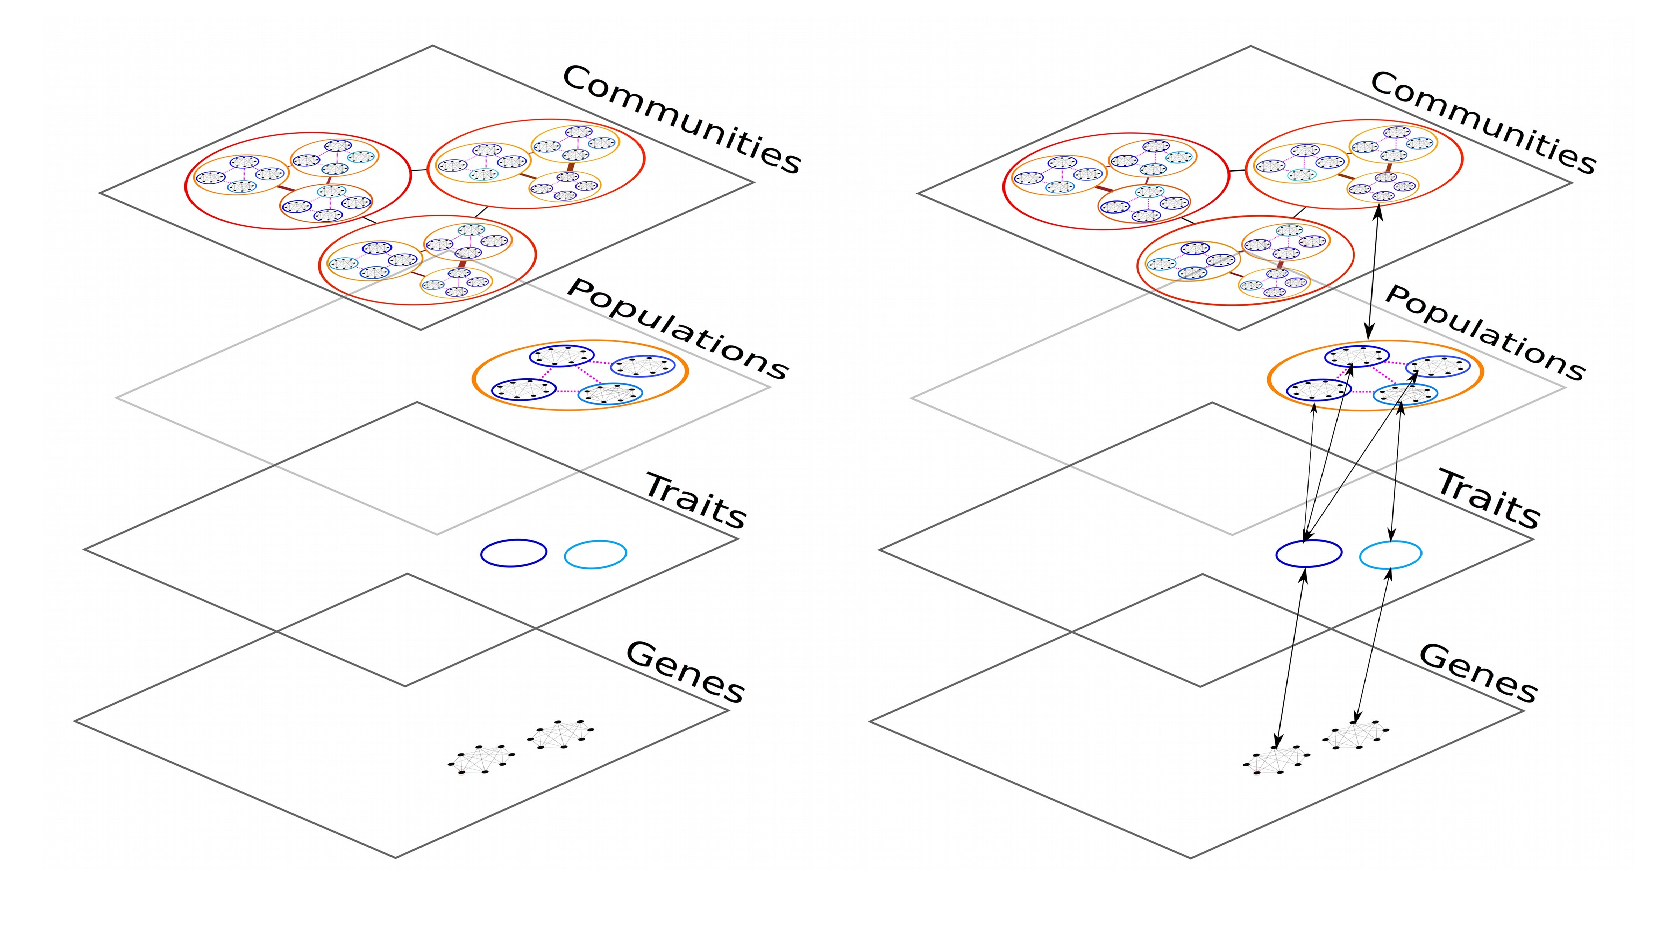
\includegraphics[height=6cm,width=11cm]{aecos.pdf}
  \end{center}
\end{beamerboxesrounded}
}

%It deals mostly with trait evolution -- rapid trait changes 
\subsection{Eco-evolutionary networks}
\frame{\frametitle{}
  \vspace{0.25 in}
\setbeamercolor{uppercol}{fg=black,bg=white}
\setbeamercolor{lowercol}{fg=black,bg=white}
\vspace{-0.5 in}
\begin{beamerboxesrounded}[upper=upperco,lower=lowercol,shadow=true]{}
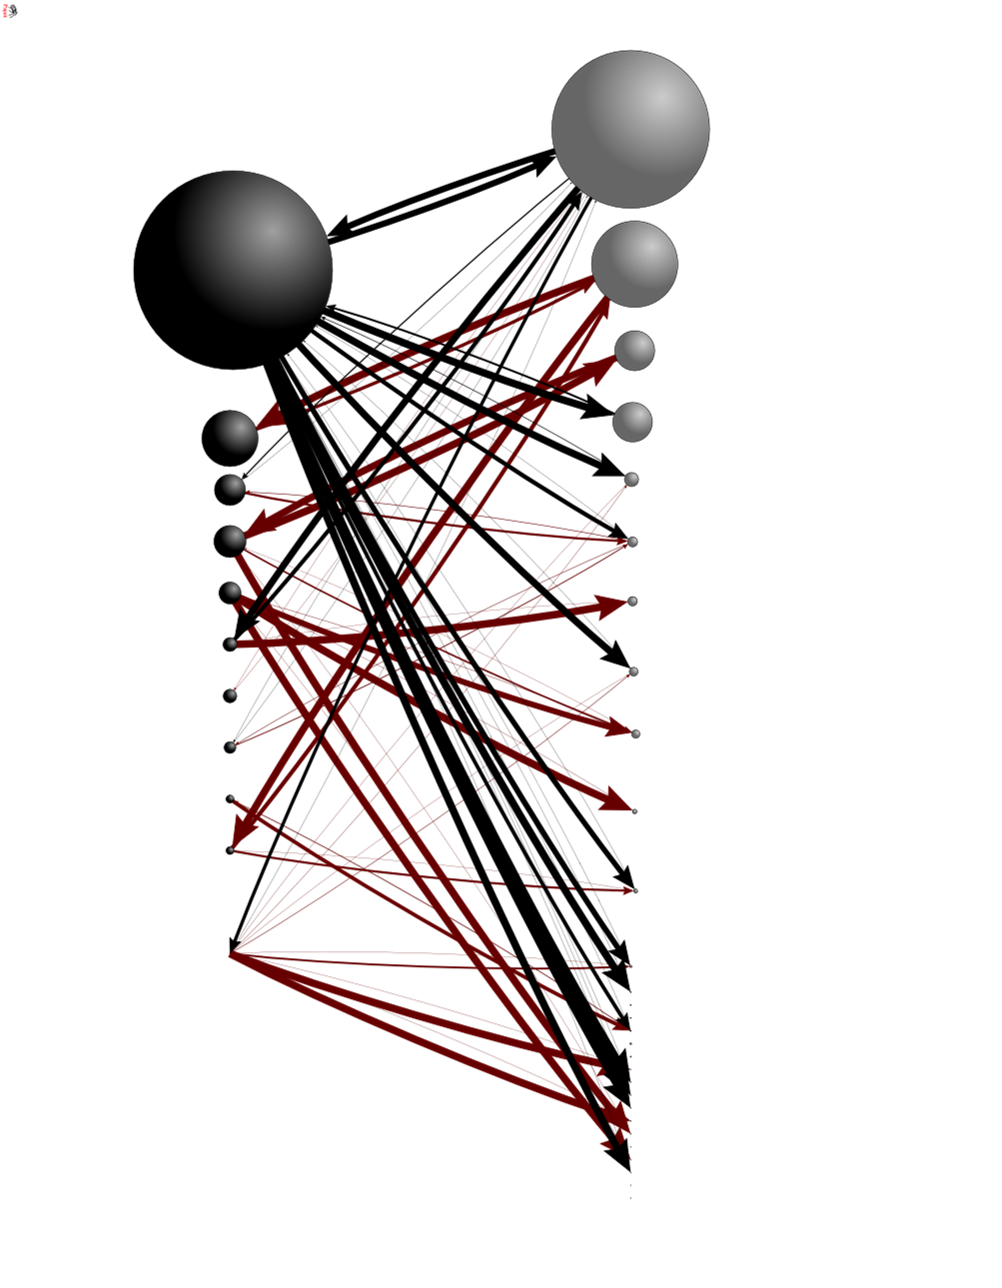
\includegraphics[height=10cm,width=7cm,angle=90]{asymmetry.png}
\end{beamerboxesrounded}
}

%It deals mostly with trait evolution -- rapid trait changes 
\subsection{Eco-evolutionary networks}
\frame{\frametitle{}
  \vspace{0.25 in}
\setbeamercolor{uppercol}{fg=black,bg=white}
\setbeamercolor{lowercol}{fg=black,bg=white}
\vspace{-0.5 in}
\begin{beamerboxesrounded}[upper=upperco,lower=lowercol,shadow=true]{}
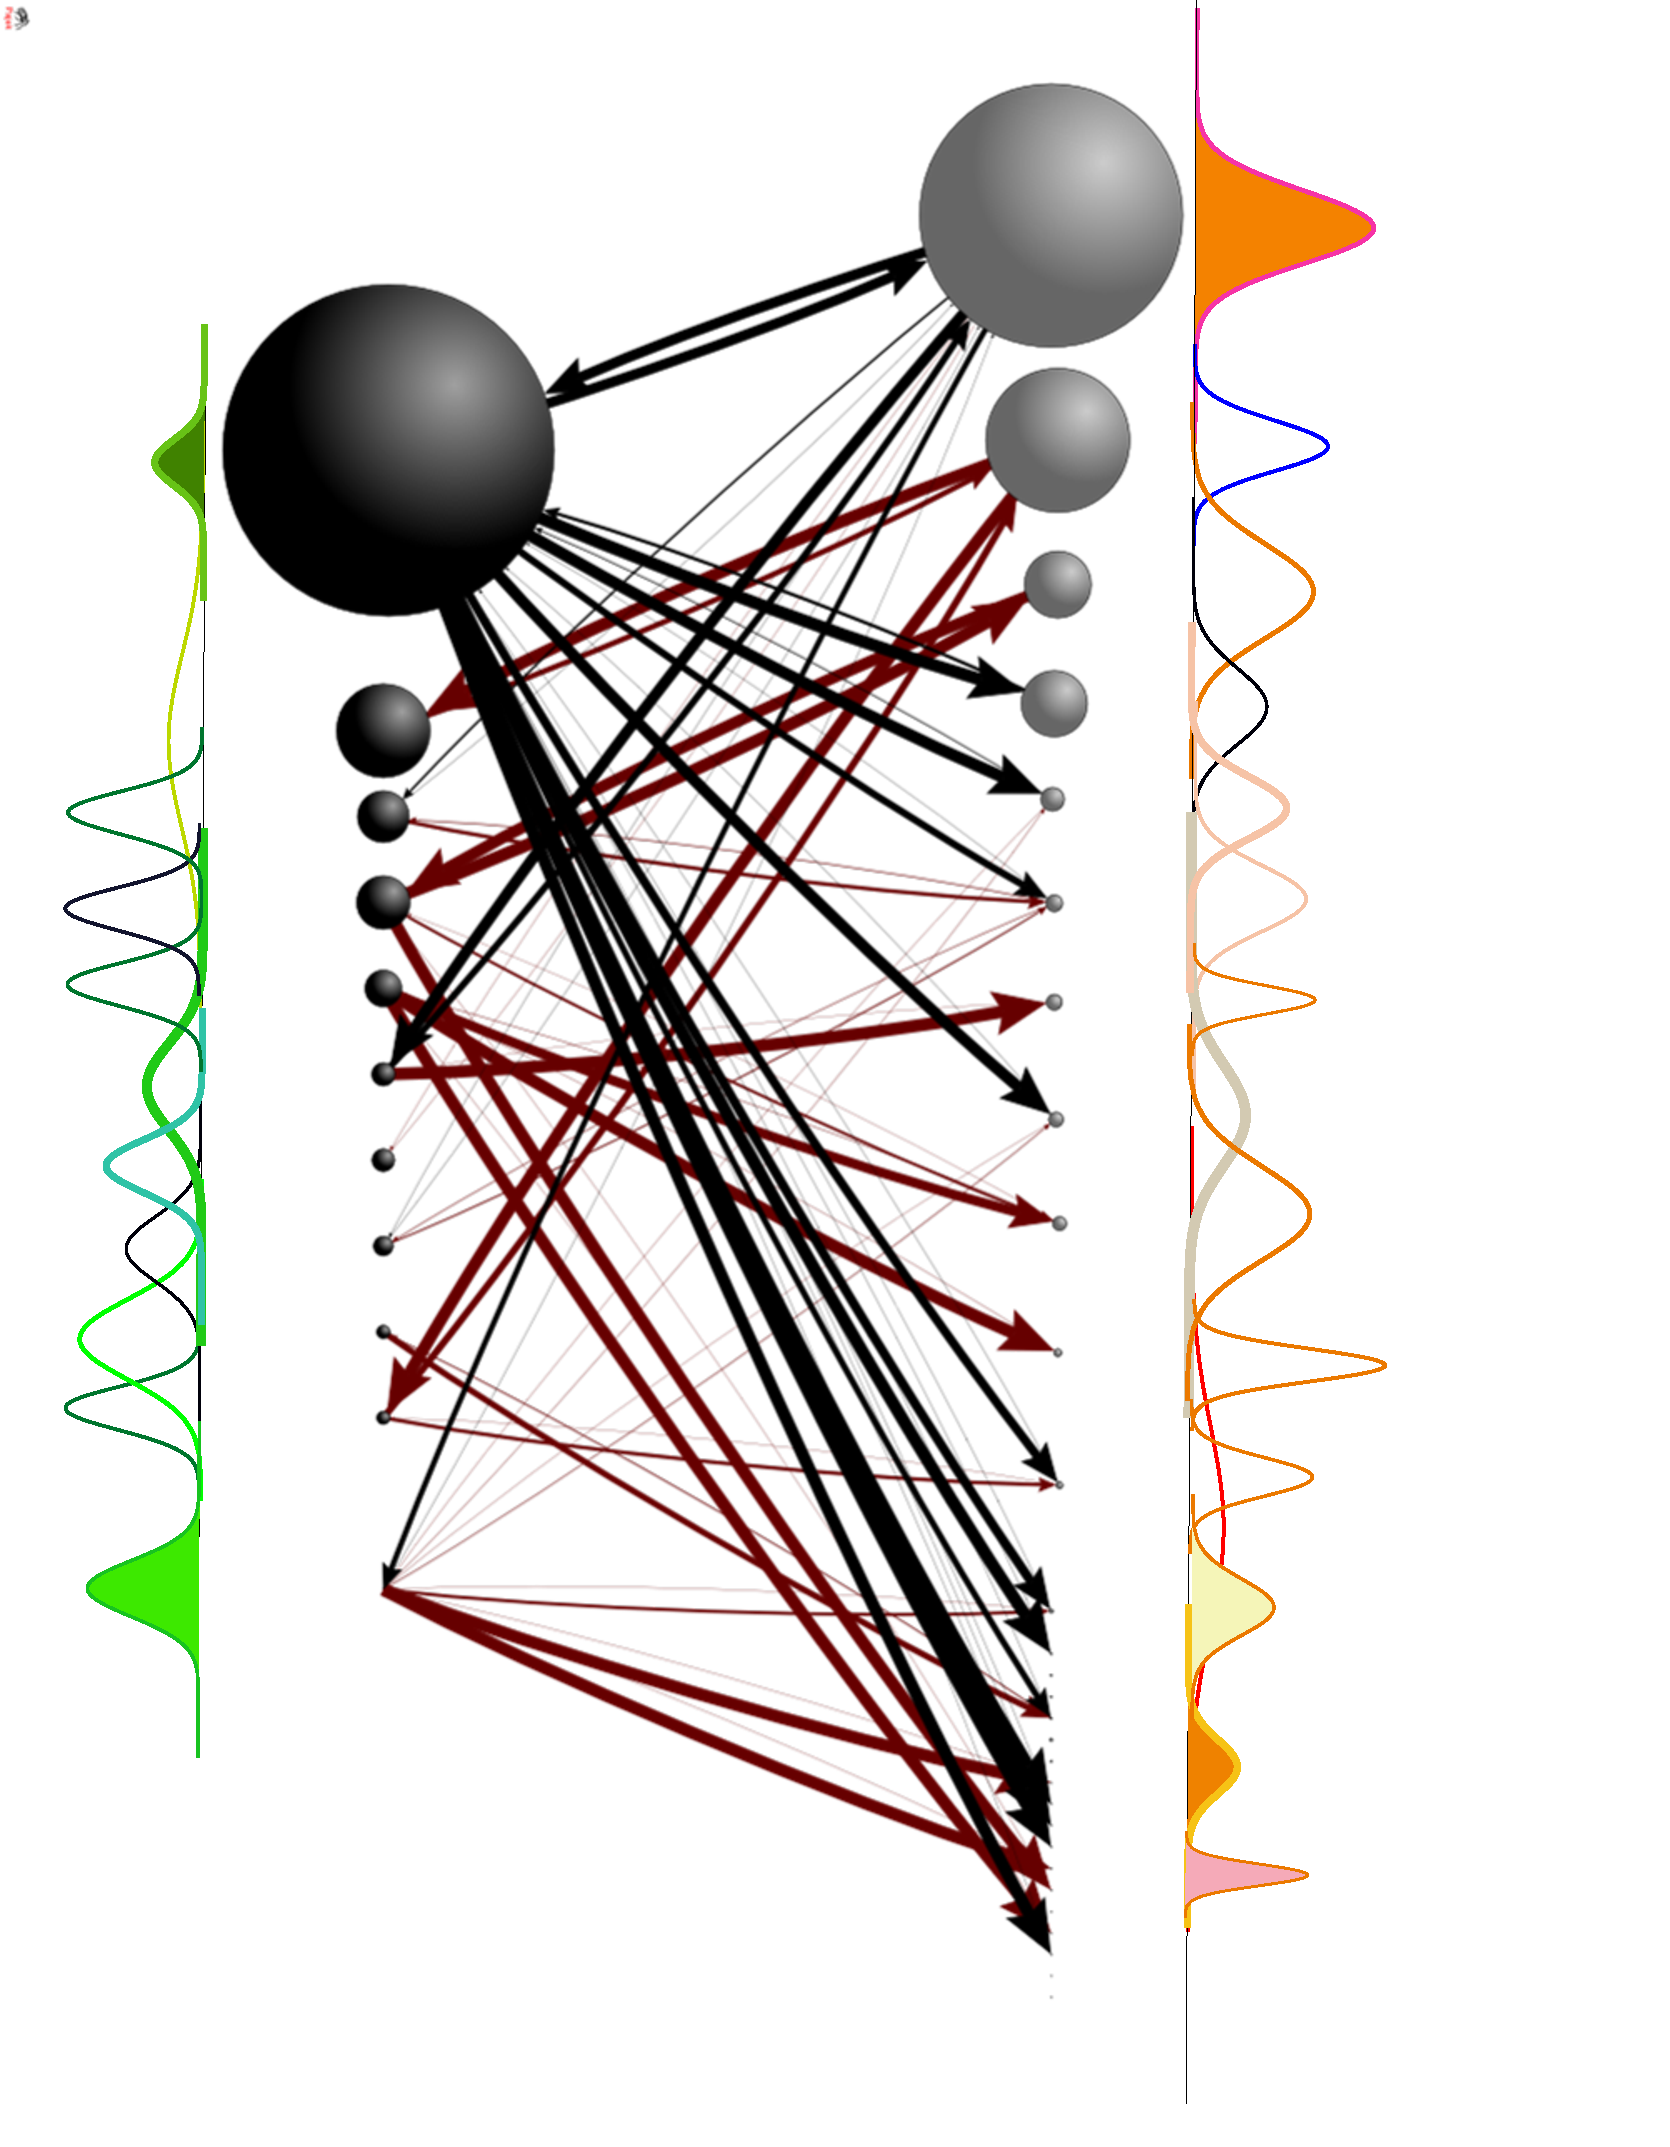
\includegraphics[height=10cm,width=7cm,angle=90]{Slide0.pdf}
\end{beamerboxesrounded}
}

%It deals mostly with trait evolution -- rapid trait changes 
\subsection{Eco-evolutionary networks}
\frame{\frametitle{}
  \vspace{0.25 in}
\setbeamercolor{uppercol}{fg=black,bg=white}
\setbeamercolor{lowercol}{fg=black,bg=white}
\vspace{-0.5 in}
\begin{beamerboxesrounded}[upper=upperco,lower=lowercol,shadow=true]{}
  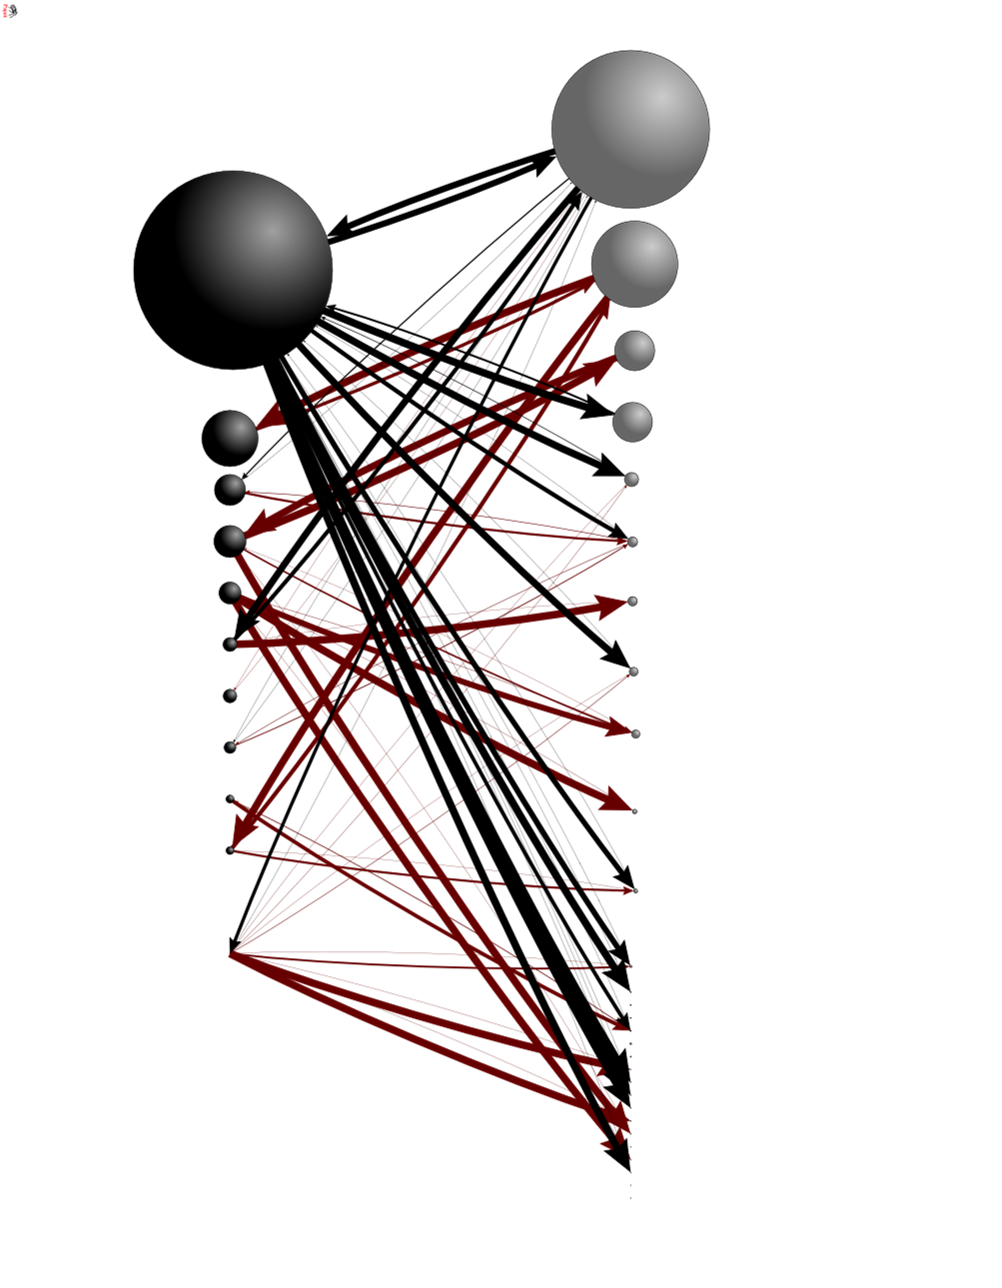
\includegraphics[height=10cm,width=7cm,angle=90]{asymmetry.png}
  \vspace{-2.77 in}
  
  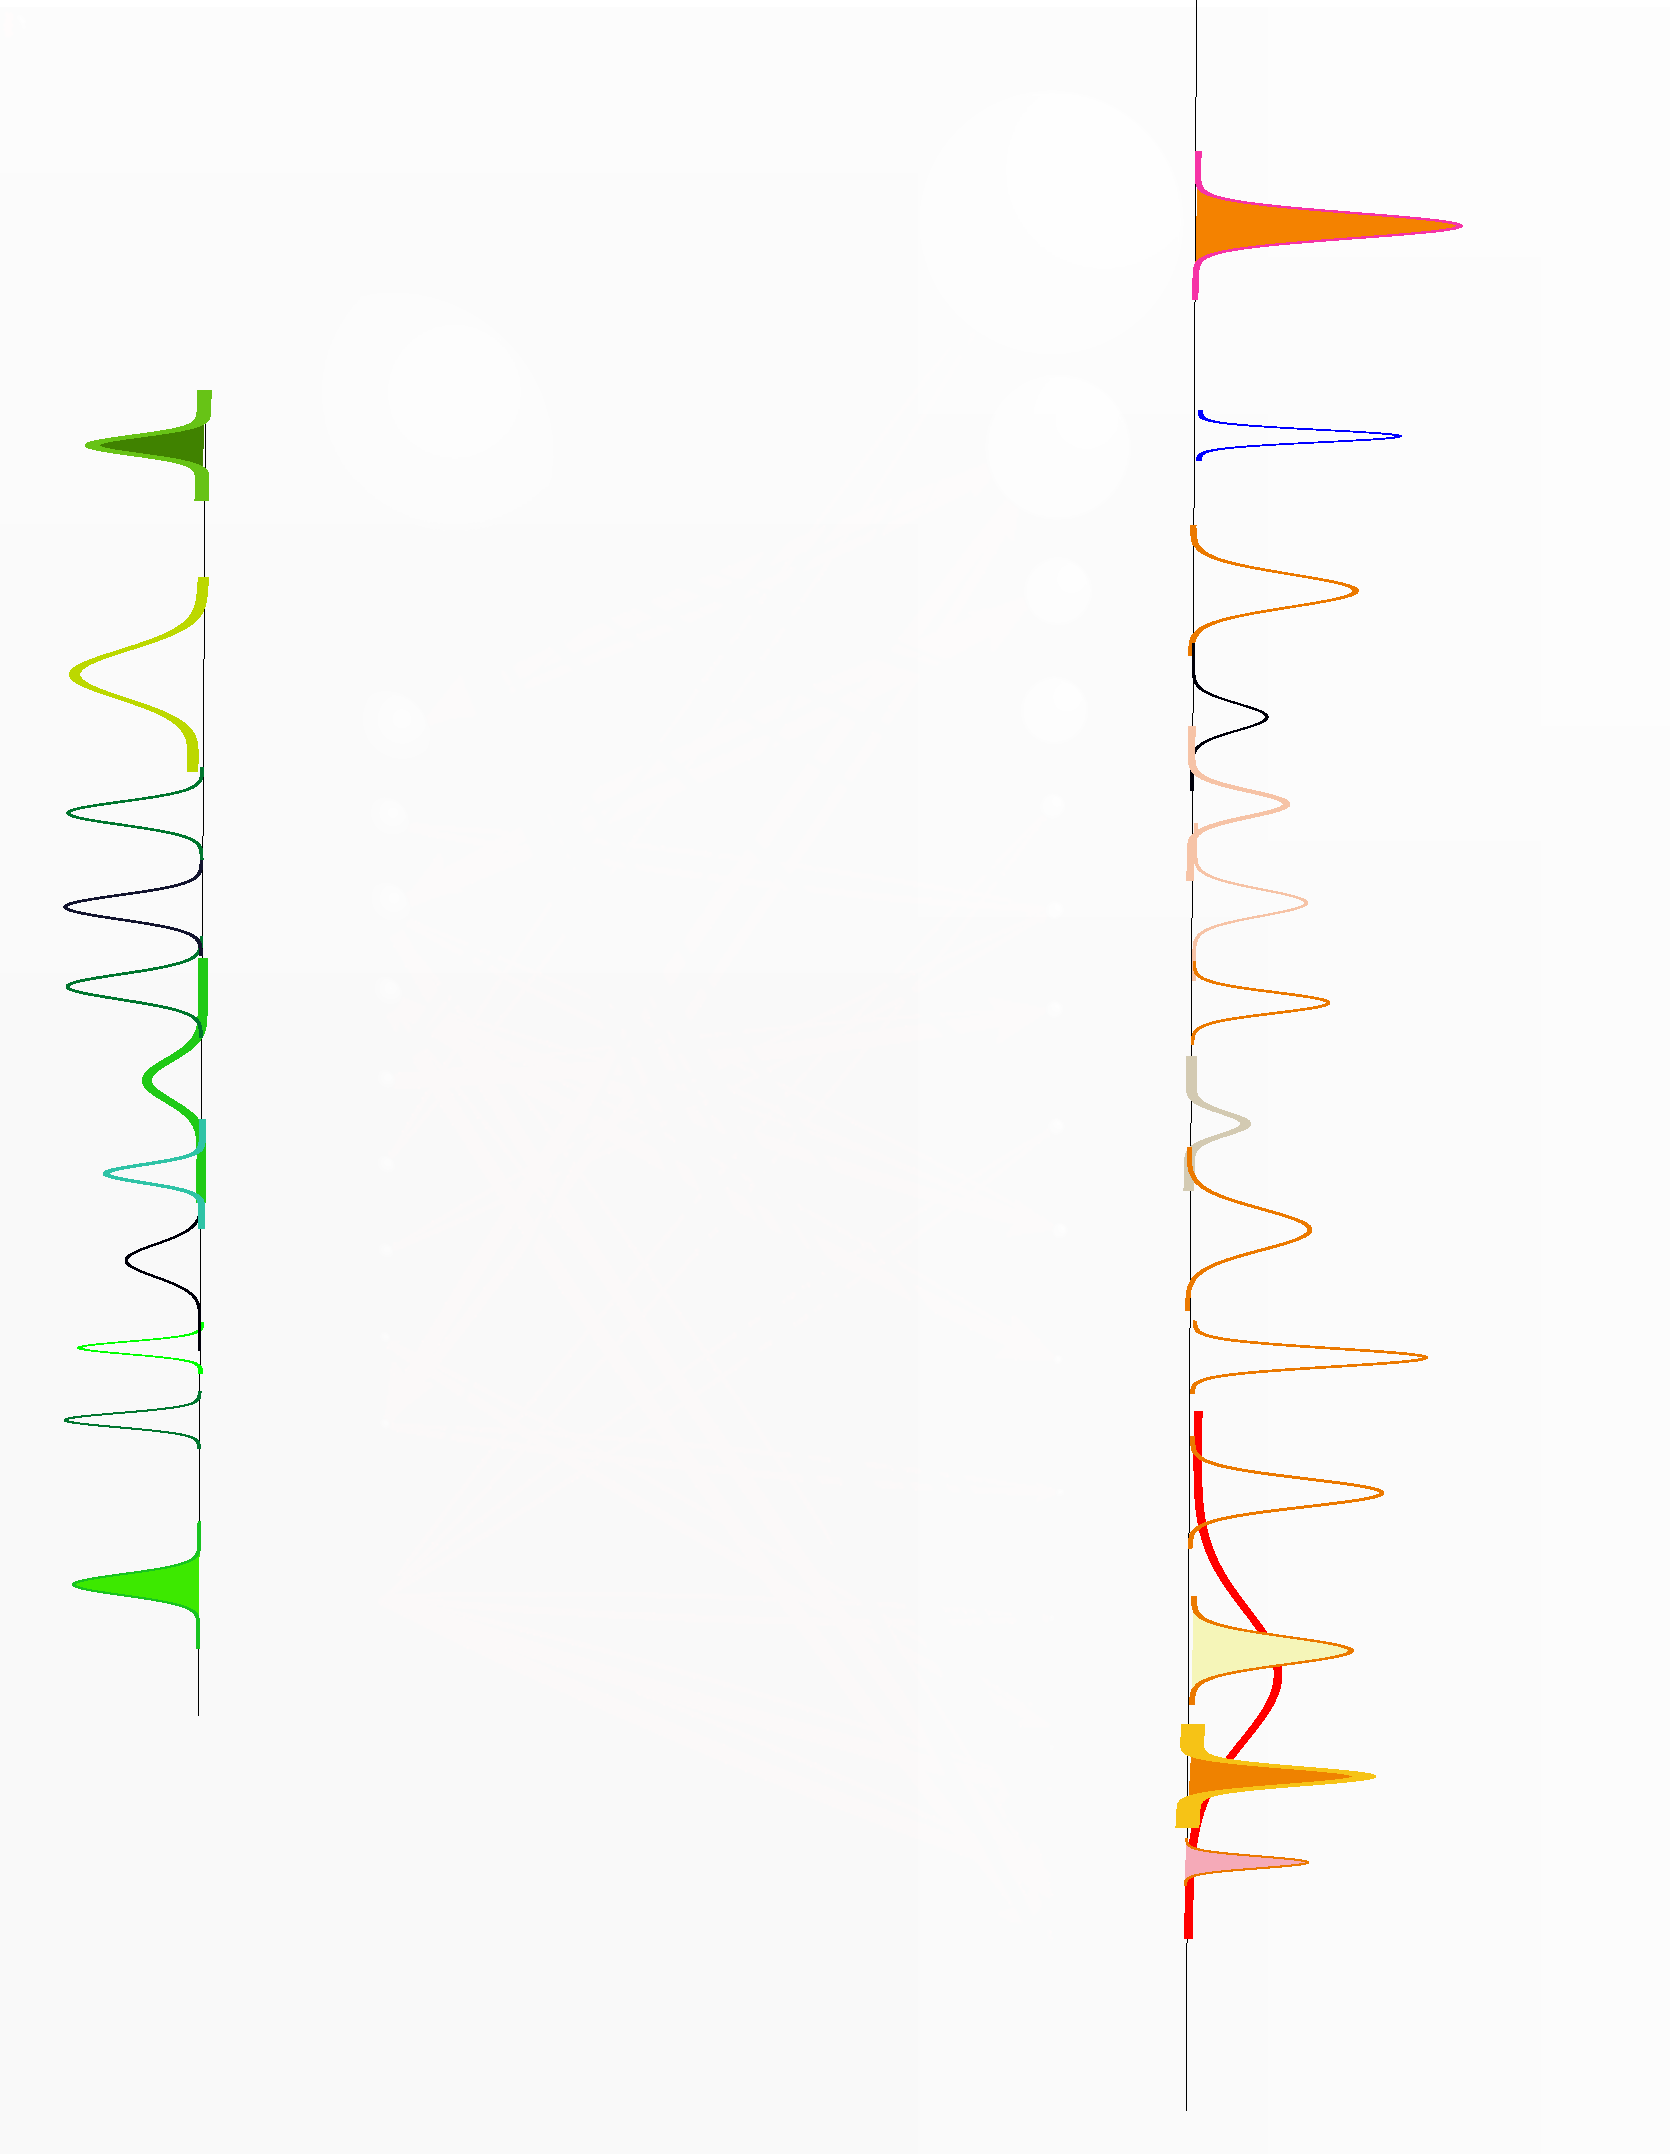
\includegraphics[height=10cm,width=7cm,angle=90]{Slide2.pdf}
\end{beamerboxesrounded}
}


\subsection{Structural stability}
\frame{\frametitle{\small{... and the architecture of traits within species might be rapidly changing}}
  \begin{center}
\vspace{0.2 in}
\hspace{-1.5 in}\includegraphics[width=12cm]{sspmn.pdf}
\end{center}
}

\section{Questions}
\subsection{Questions}
\frame{\frametitle{}
  \vspace{-1 in}
  \begin{itemize}
  \item < 1-| alert@1 > How does trait evolution affect ecological networks?
  \item < 2-| alert@2 > When and how do trait evolution and ecological networks feedback each other?
  \item < 3-| alert@3 > Which are the consequences of eco-evolutionary feedbacks for species coexistence?
\end{itemize}
}

\section{Model systems}

% ------------------------Cichlids-----------------------------------------------------------
\subsection{Eco-evolutionary tangling I}
\frame{\frametitle{\small{... radiations can be rapid}}
  \begin{center}
\vspace{-0.2 in}
\hspace{-0.5 in}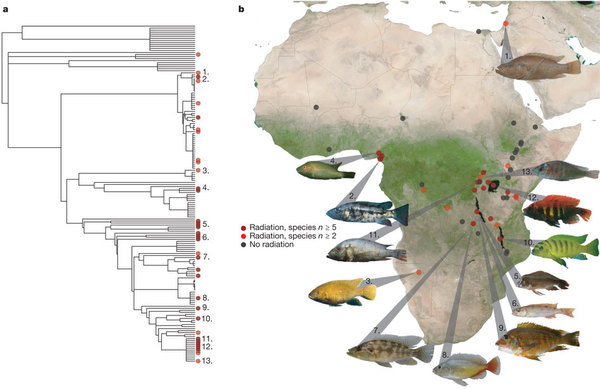
\includegraphics[width=9cm]{biogeographyradiations.png}
\end{center}
}


\subsection{Eco-evolutionary tangling II}
\frame{\frametitle{\small{... meaning ecological and evolutionary dynamics might be tangled}}
    \vspace{-0.2 in}
\begin{columns}
    \begin{column}{6cm}
    \hspace{0.25 in}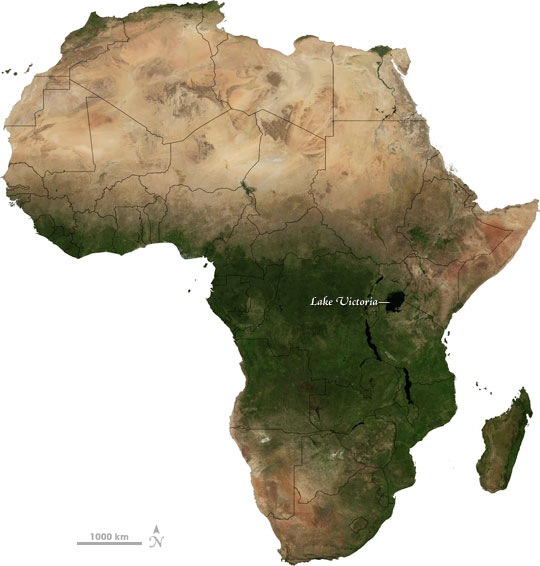
\includegraphics[width=5cm]{LVictoria.jpg}
    \end{column}
      
    \begin{column}{6cm}
    \hspace{-0.25 in}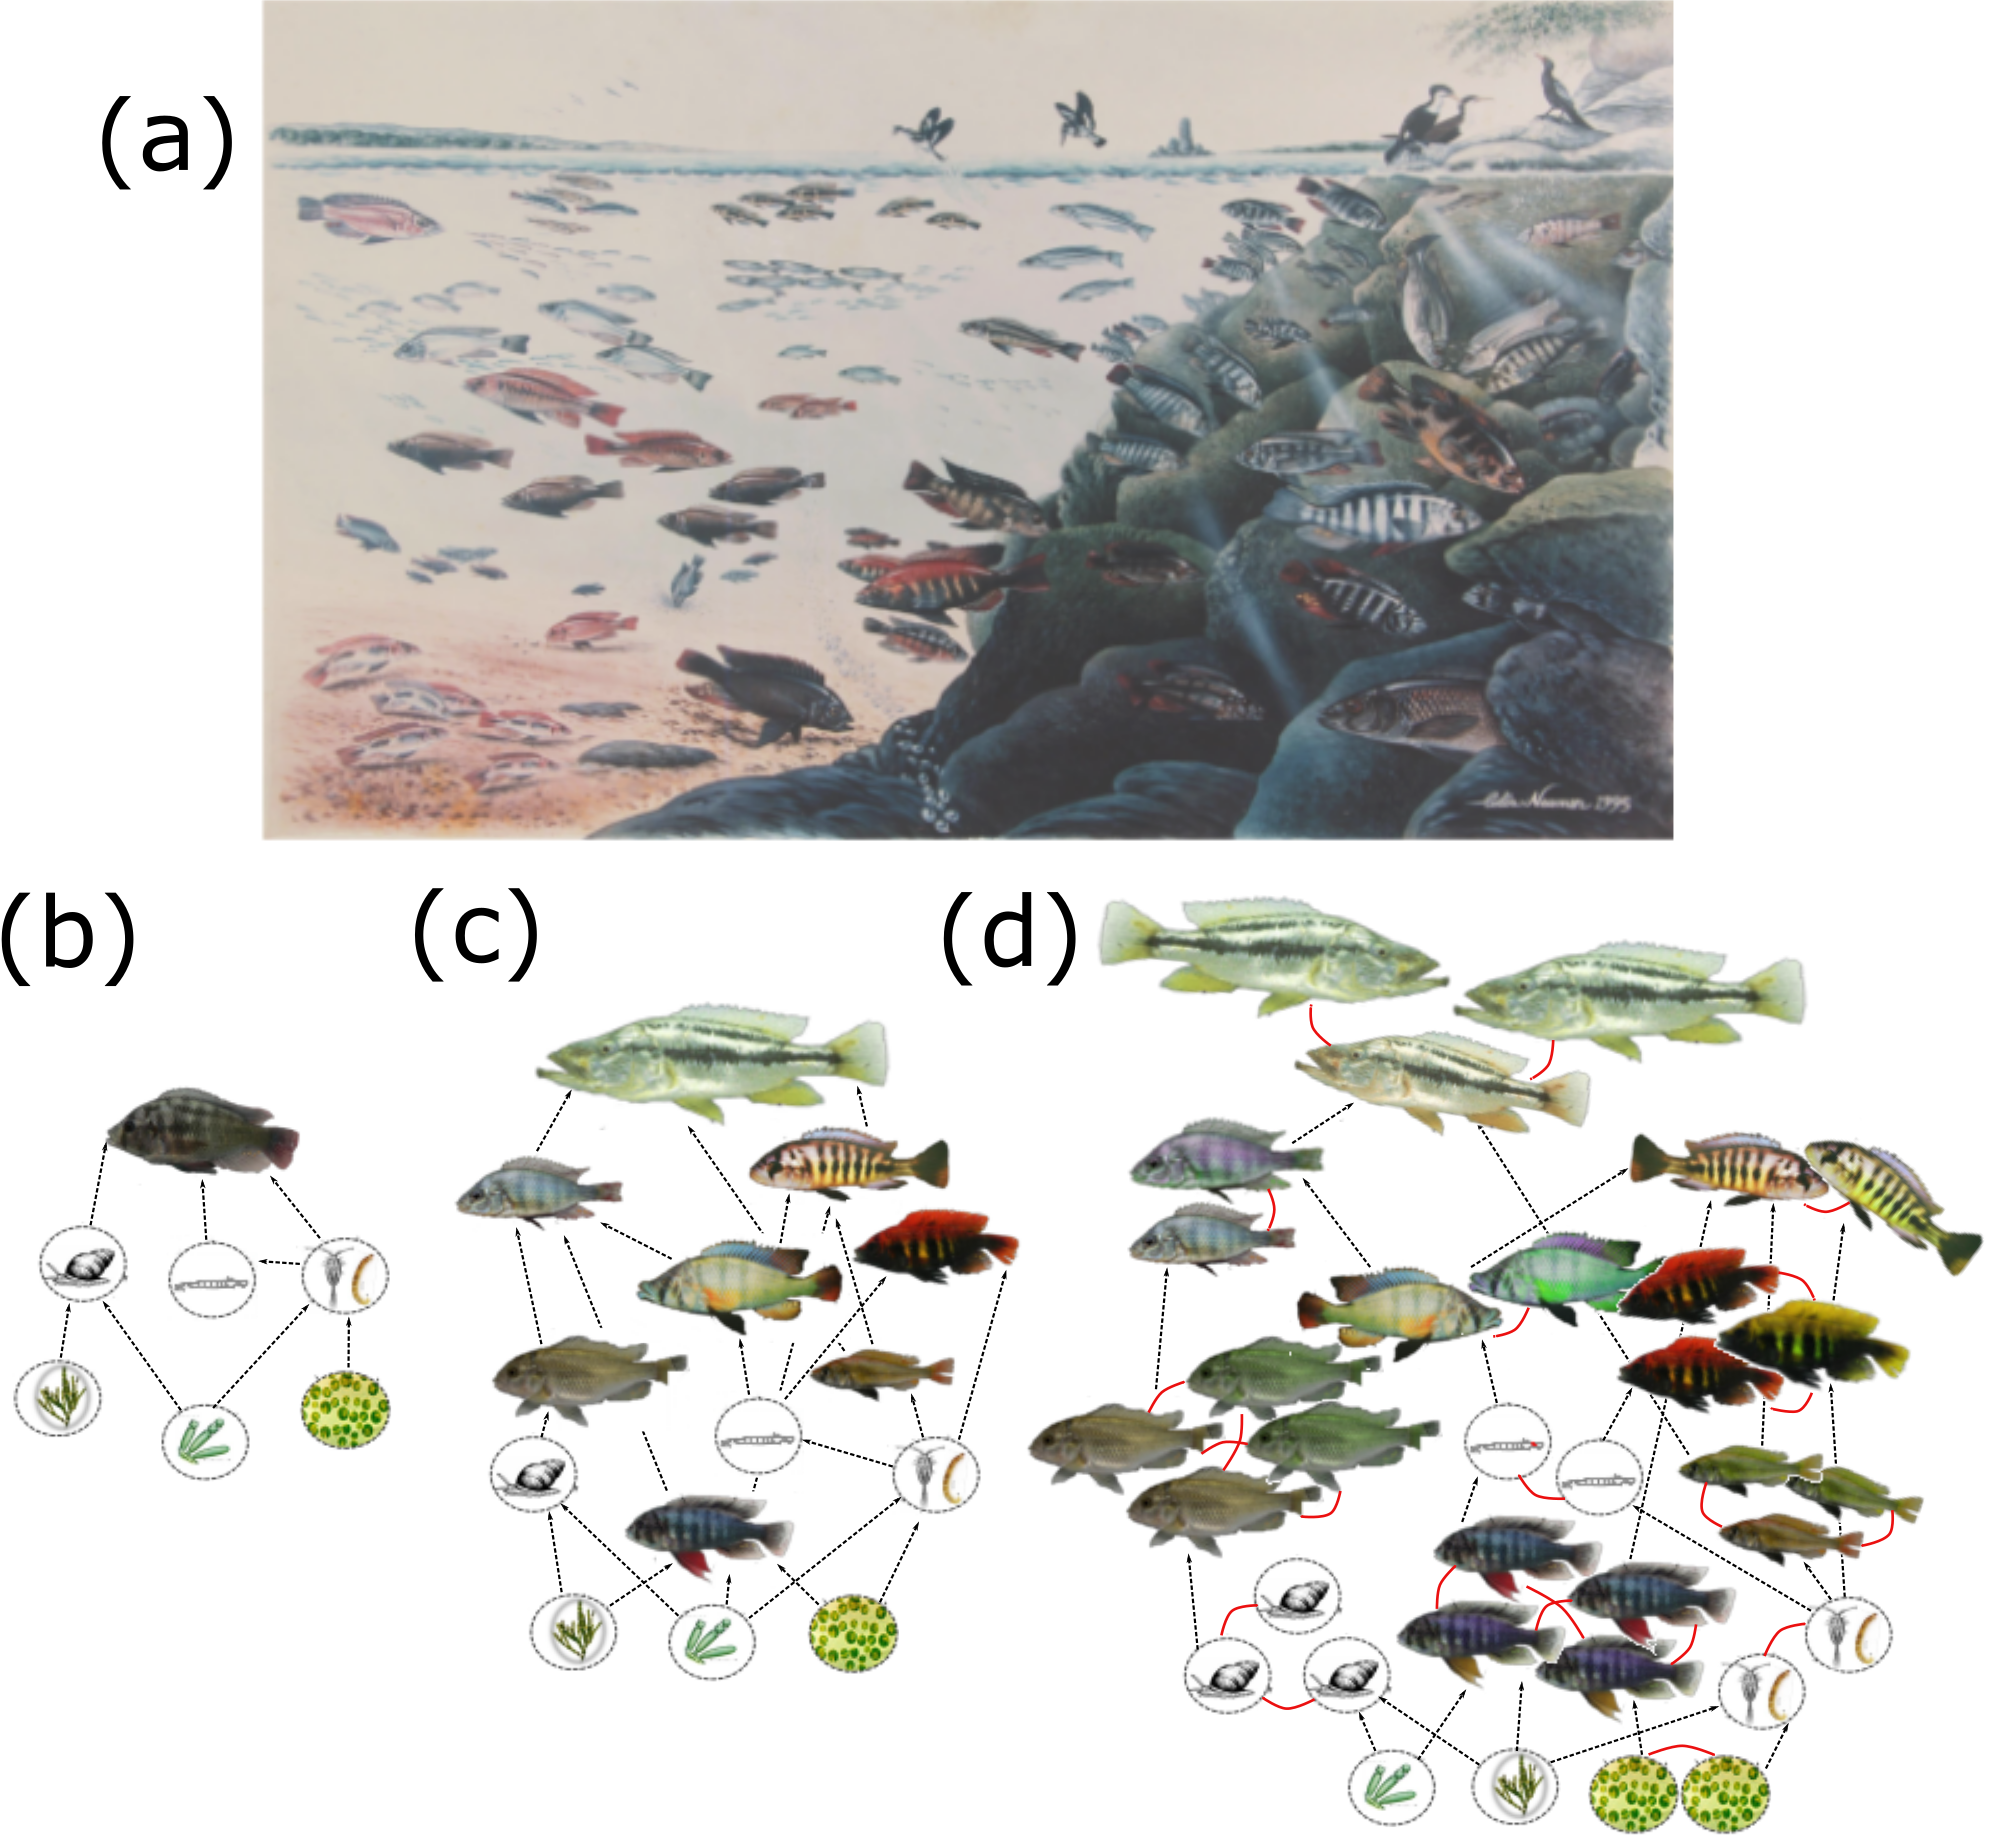
\includegraphics[width=6cm]{cichlids.png}
    \end{column}

\end{columns}
}
%------------------------------------------------------------------------------------------


%---------------------------Sticklebacks----------------------------------------------------
\subsection{Model system I}
\frame{\frametitle{\small{Sticklebacks}}
\setbeamercolor{uppercol}{fg=black,bg=white}
\setbeamercolor{lowercol}{fg=black,bg=white}
\begin{beamerboxesrounded}[upper=upperco,lower=lowercol,shadow=true]{}
    \vspace{-1.25 in}
    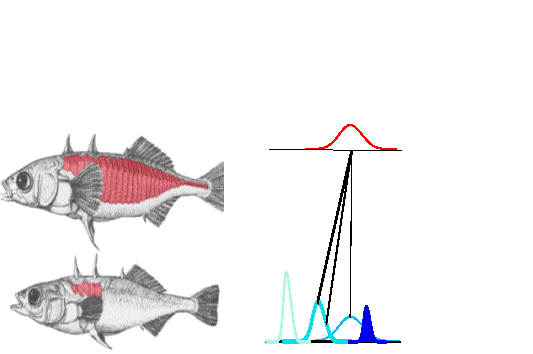
\includegraphics[height=6cm,width=11cm]{Sticklebacks.pdf}
\end{beamerboxesrounded}
}
%Enrich biology
%http://blog.targethealth.com/2007/12/17/

%effects from
%https://tex.stackexchange.com/questions/204522/letter-by-letter-uncovering-animation-effect
%-------------------------------------------------------------------------------------------


%======================================================
\subsection{Model system II}
\frame{\frametitle{\small{Darwin's finches I}}
\setbeamercolor{uppercol}{fg=black,bg=white}
\setbeamercolor{lowercol}{fg=black,bg=white}
\begin{beamerboxesrounded}[upper=upperco,lower=lowercol,shadow=true]{}
\begin{center}
\vspace{0.1 in}
\hspace{-2 in}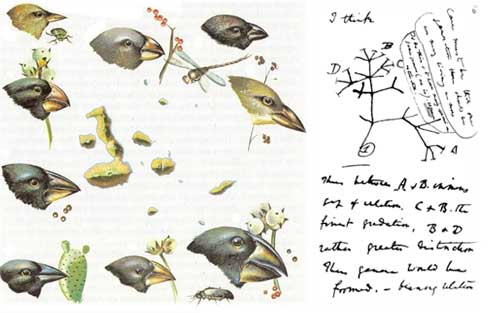
\includegraphics[height=4cm,width=5cm]{BeakIslands.png}
\end{center}
\begin{center}
\vspace{-1.75 in}
\hspace{2 in}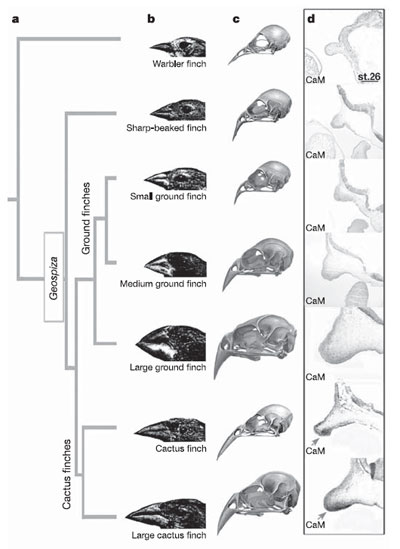
\includegraphics[height=6cm,width=5cm]{Darwinbeak.png}\footnotetext{{\Tiny Abzhanov, A., et. al
    (2006). The calmodulin pathway and evolution of elongated beak morphology in Darwin's finches, Nature, 442:563-567.}}
\end{center}
\end{beamerboxesrounded}
}


\subsection{Model system II}
\frame{\frametitle{\small{Darwin's finches II}}
\vspace{0.25 in}
  \setbeamercolor{uppercol}{fg=black,bg=white}
\setbeamercolor{lowercol}{fg=black,bg=white}
\begin{beamerboxesrounded}[upper=upperco,lower=lowercol,shadow=true]{}
      \hspace{-0.15 in}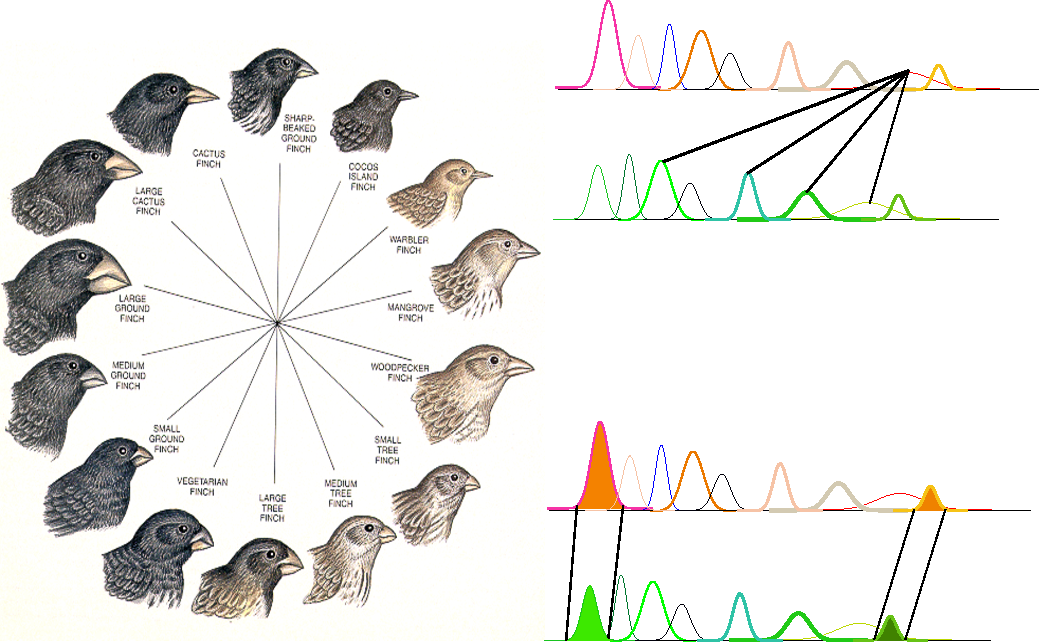
\includegraphics[height=6cm,width=11cm]{darwinv1.pdf}
\end{beamerboxesrounded}
}

%======================================================

%Theoretical examples
\section{Eco-evolutionary networks}


\subsection{Modeling strategies}
\frame{\frametitle{}
\setbeamercolor{uppercol}{fg=black,bg=white}
\setbeamercolor{lowercol}{fg=black,bg=white}
\begin{beamerboxesrounded}[upper=upperco,lower=lowercol,shadow=true]{}
\hspace{-0.5 in}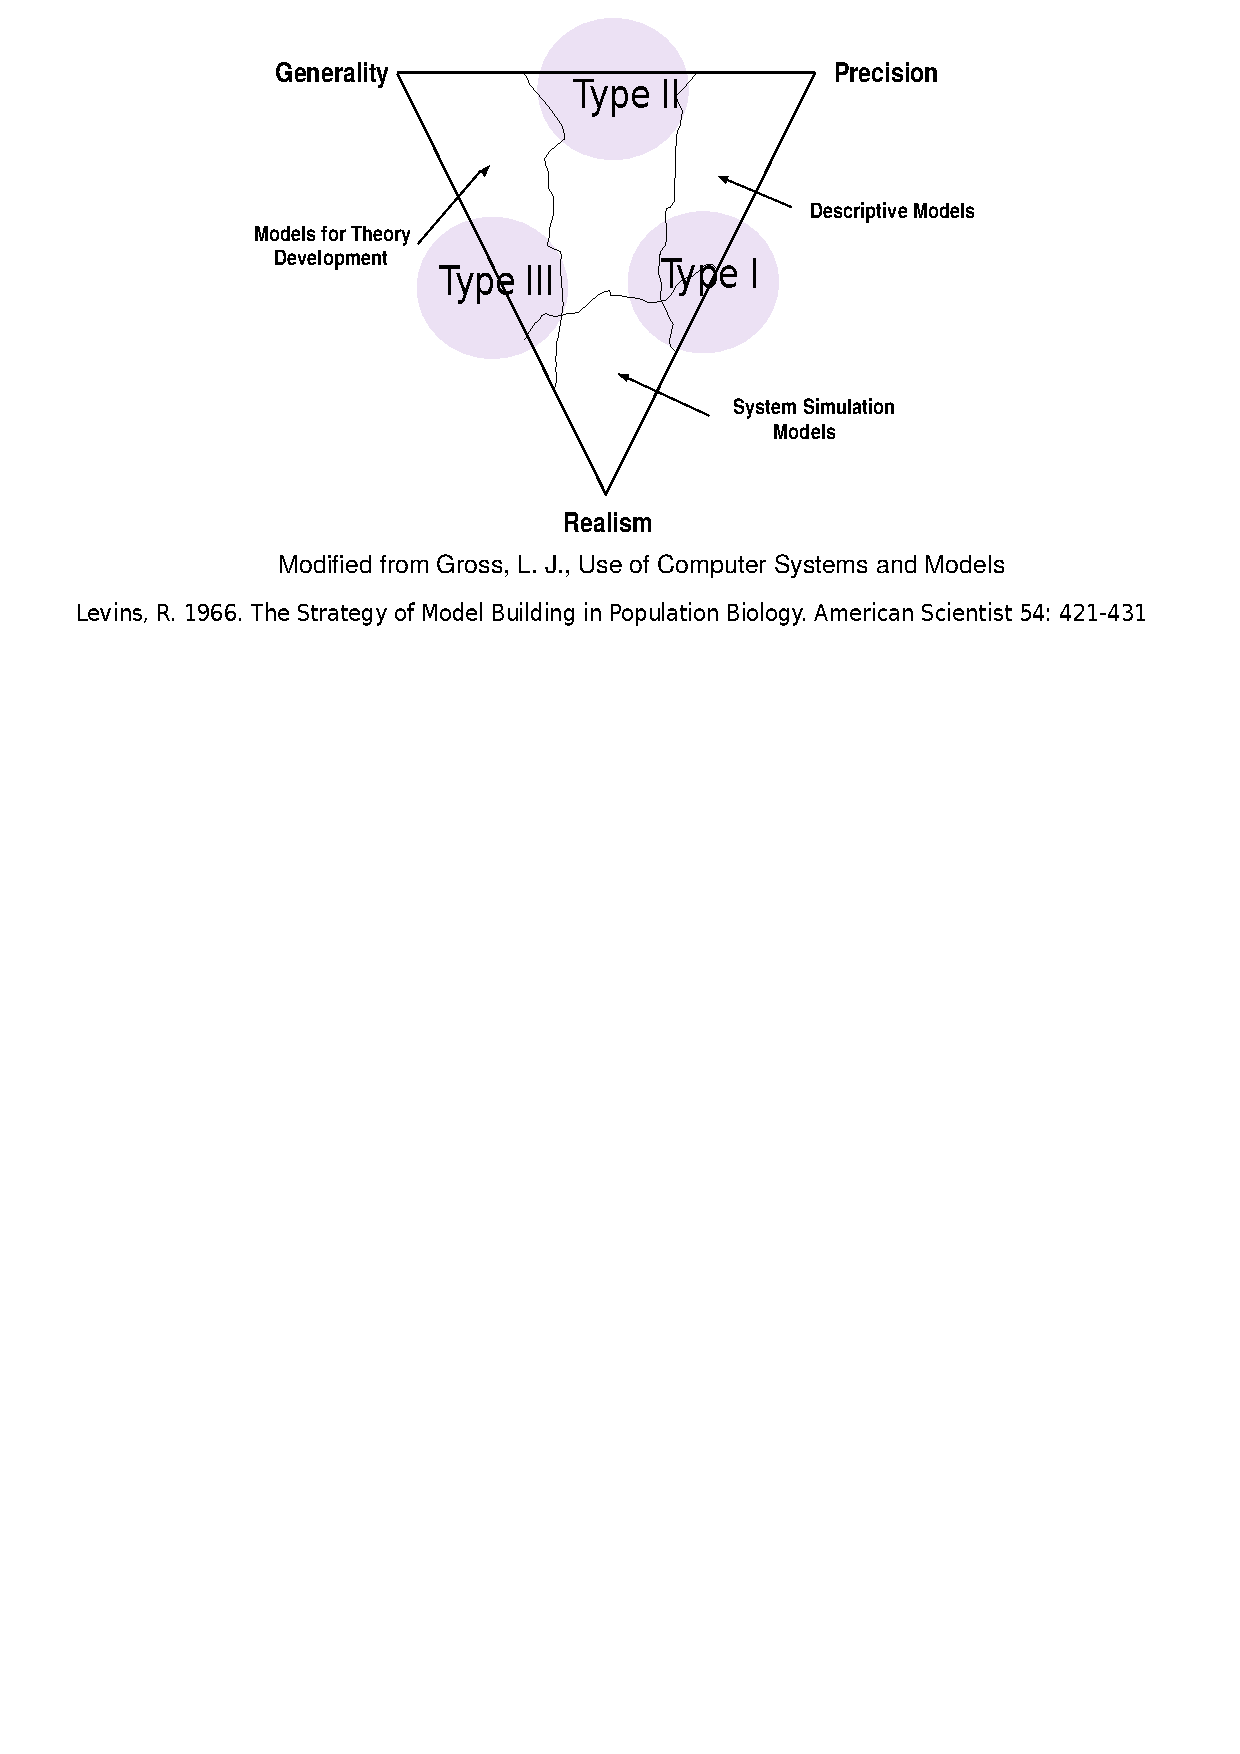
\includegraphics[width=12cm]{TradeOffs.pdf}
\end{beamerboxesrounded}
}

%It deals mostly with trait evolution -- rapid trait changes 
\subsection{Eco-evolutionary networks}
\frame{\frametitle{}
  \vspace{0.25 in}
\setbeamercolor{uppercol}{fg=black,bg=white}
\setbeamercolor{lowercol}{fg=black,bg=white}
\vspace{-0.5 in}
\begin{beamerboxesrounded}[upper=upperco,lower=lowercol,shadow=true]{}
  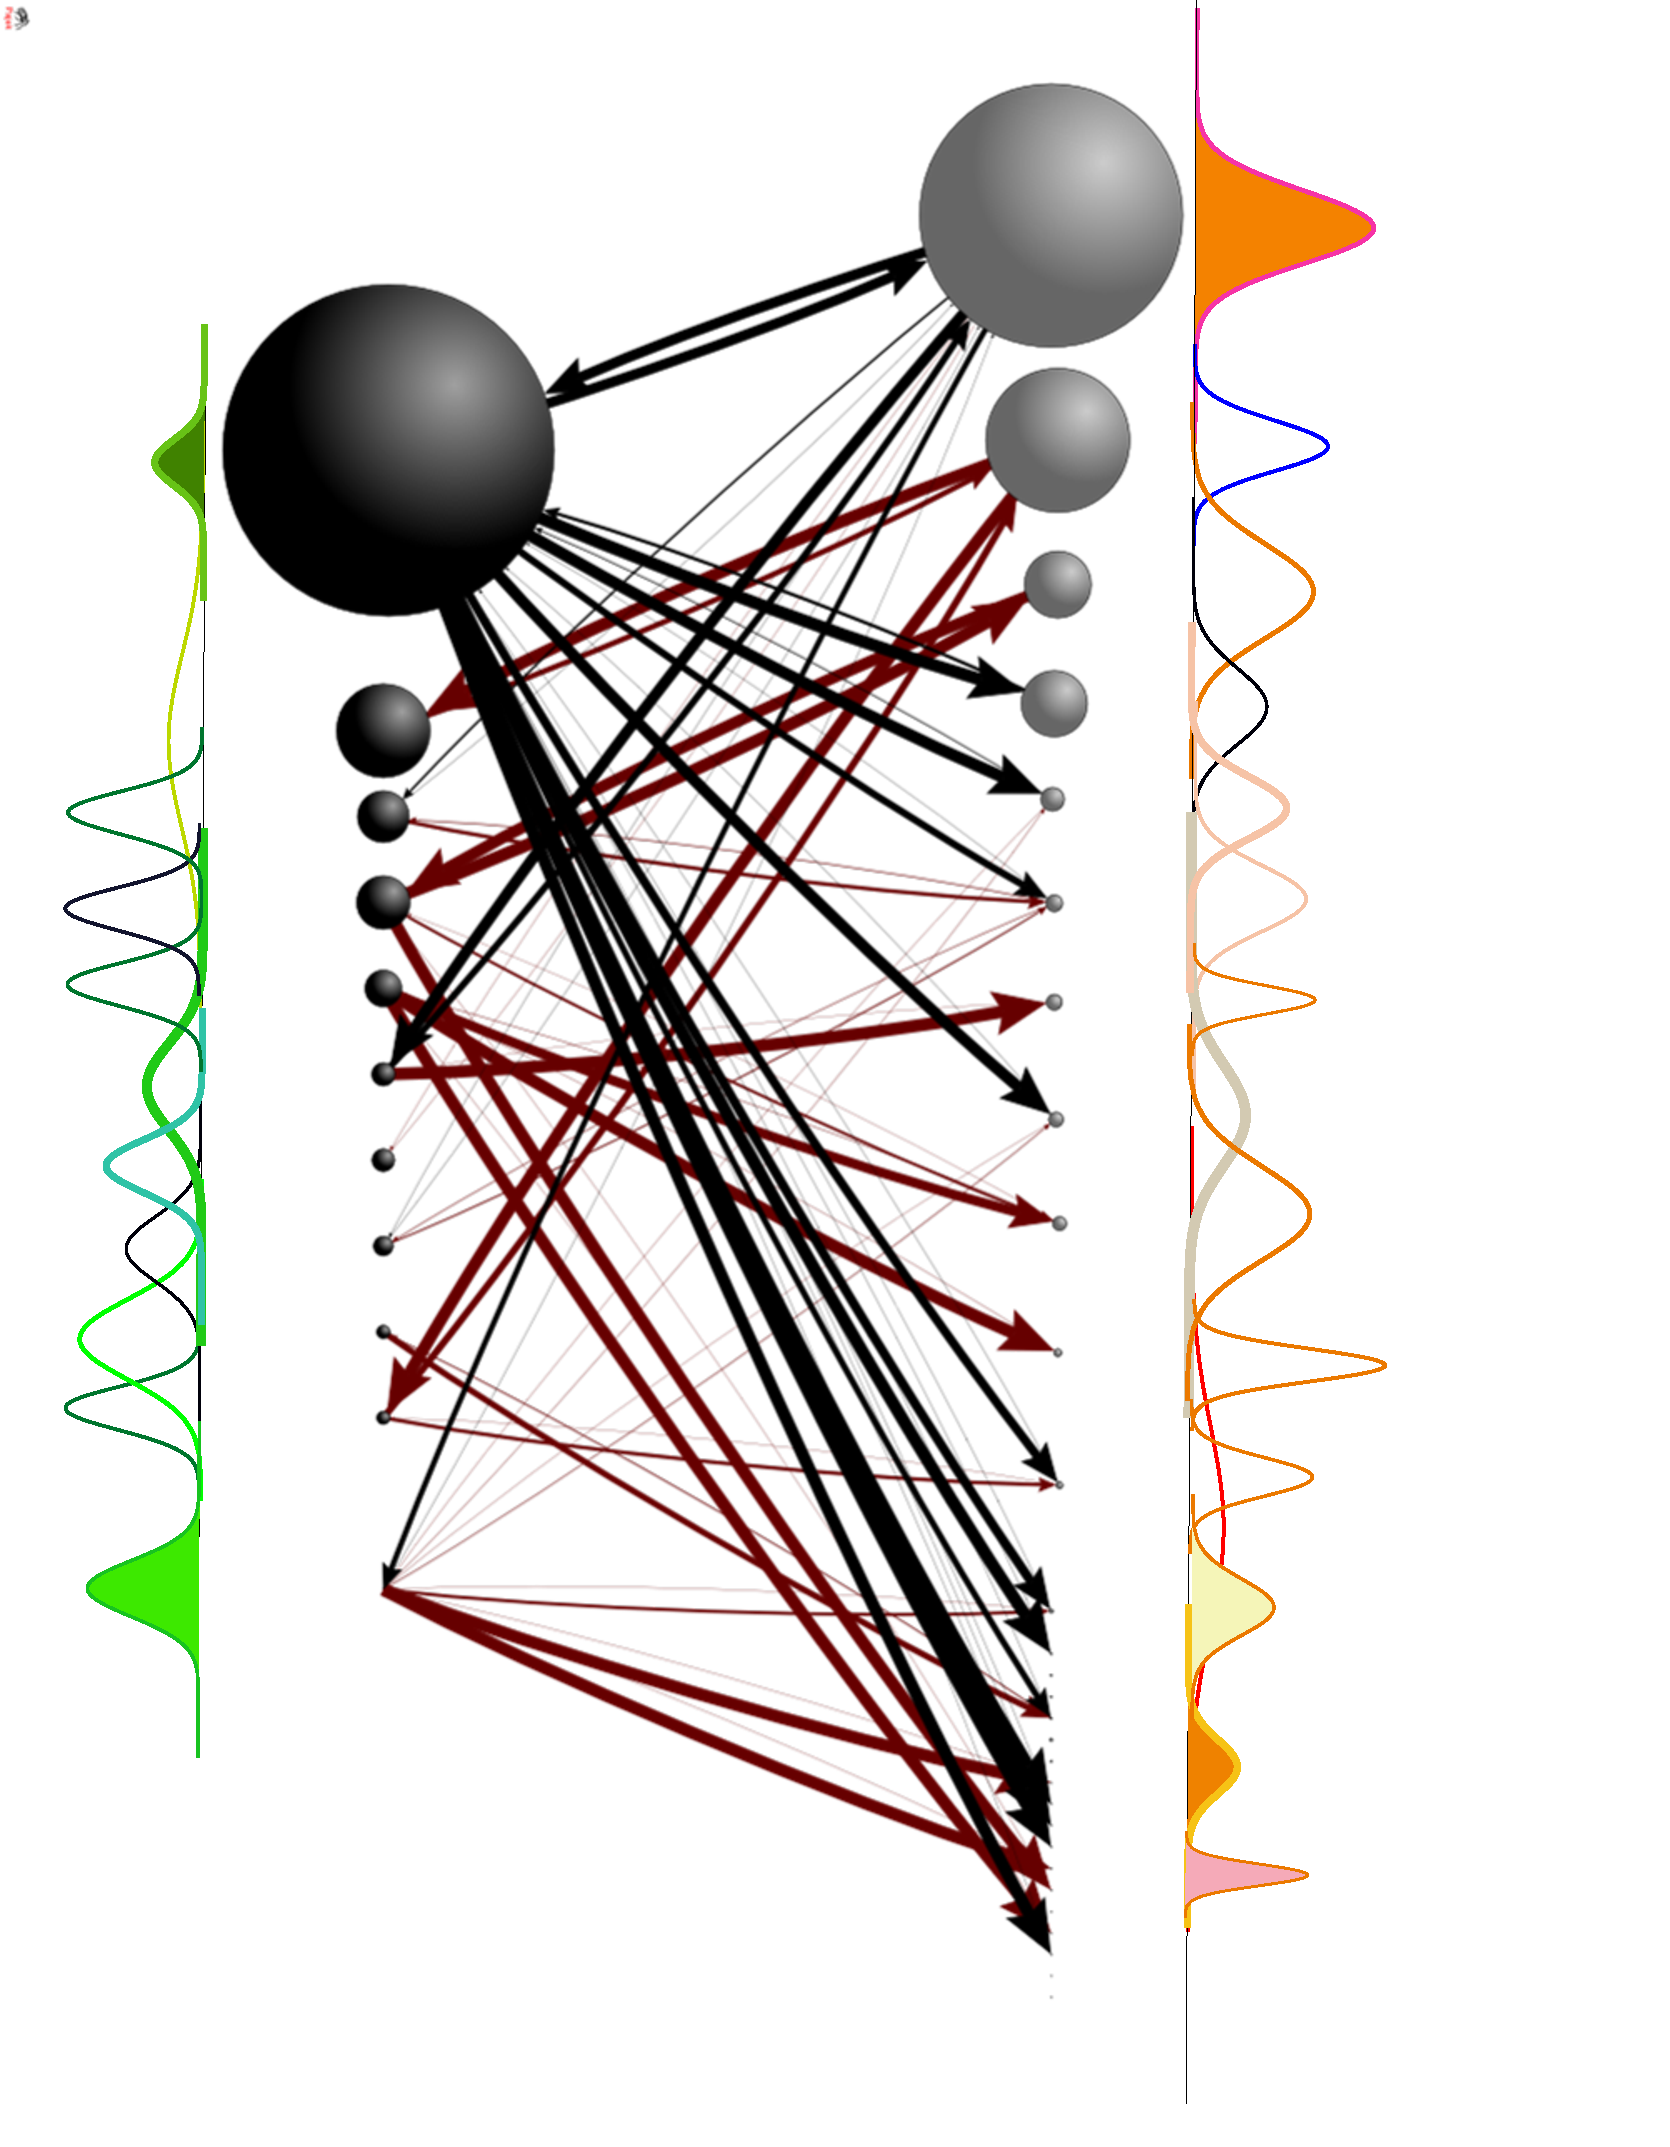
\includegraphics[height=10cm,width=7cm,angle=90]{Slide0.pdf}
\end{beamerboxesrounded}
}


%It deals mostly with trait evolution -- rapid trait changes 
\subsection{Eco-evolutionary networks}
\frame{\frametitle{}
  \vspace{0.25 in}
\setbeamercolor{uppercol}{fg=black,bg=white}
\setbeamercolor{lowercol}{fg=black,bg=white}
\vspace{-0.5 in}
\begin{beamerboxesrounded}[upper=upperco,lower=lowercol,shadow=true]{}
  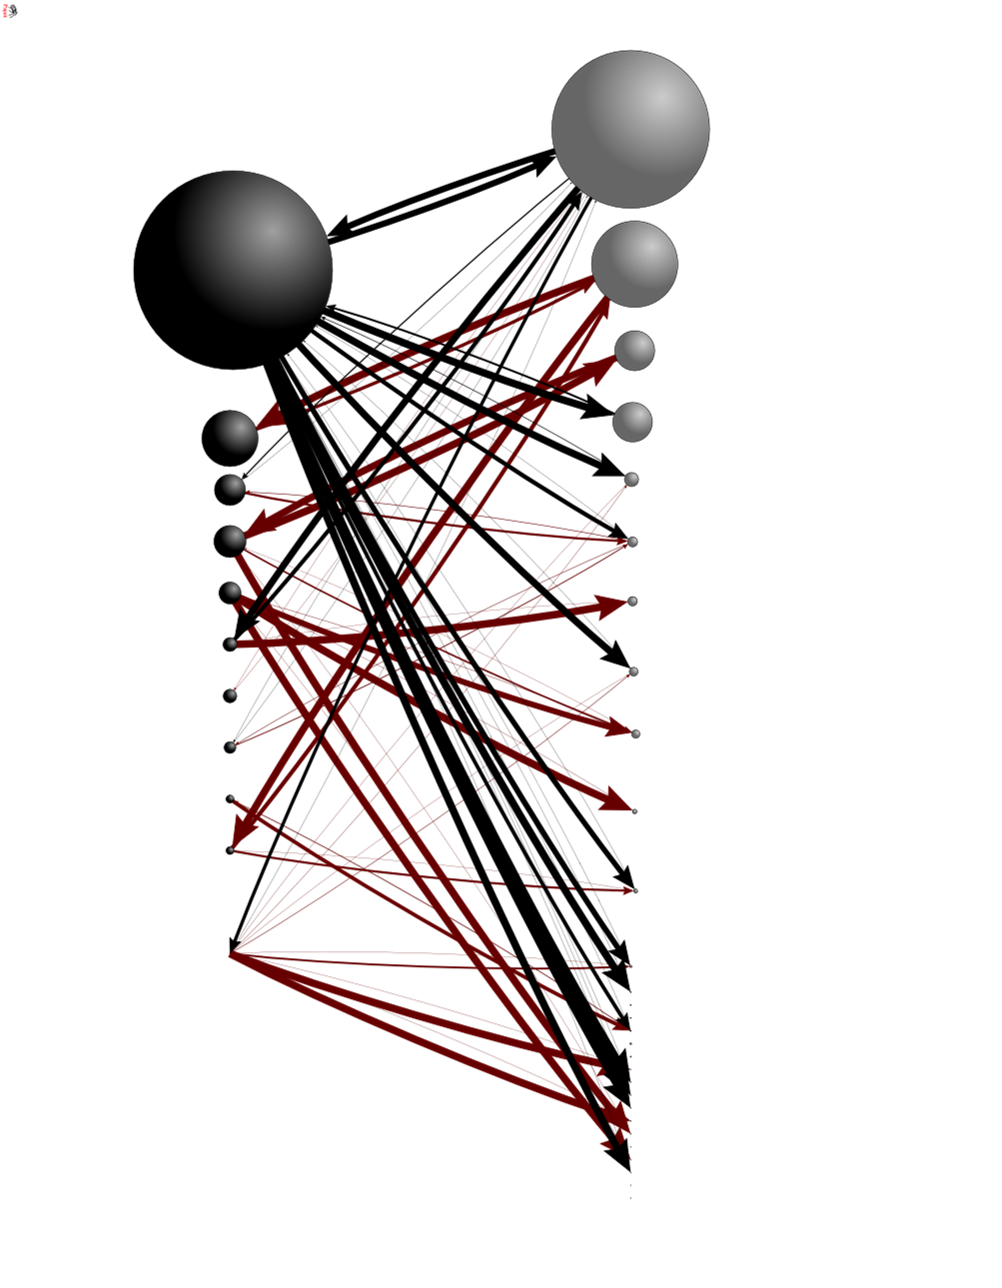
\includegraphics[height=10cm,width=7cm,angle=90]{asymmetry.png}
  \vspace{-2.77 in}
  
  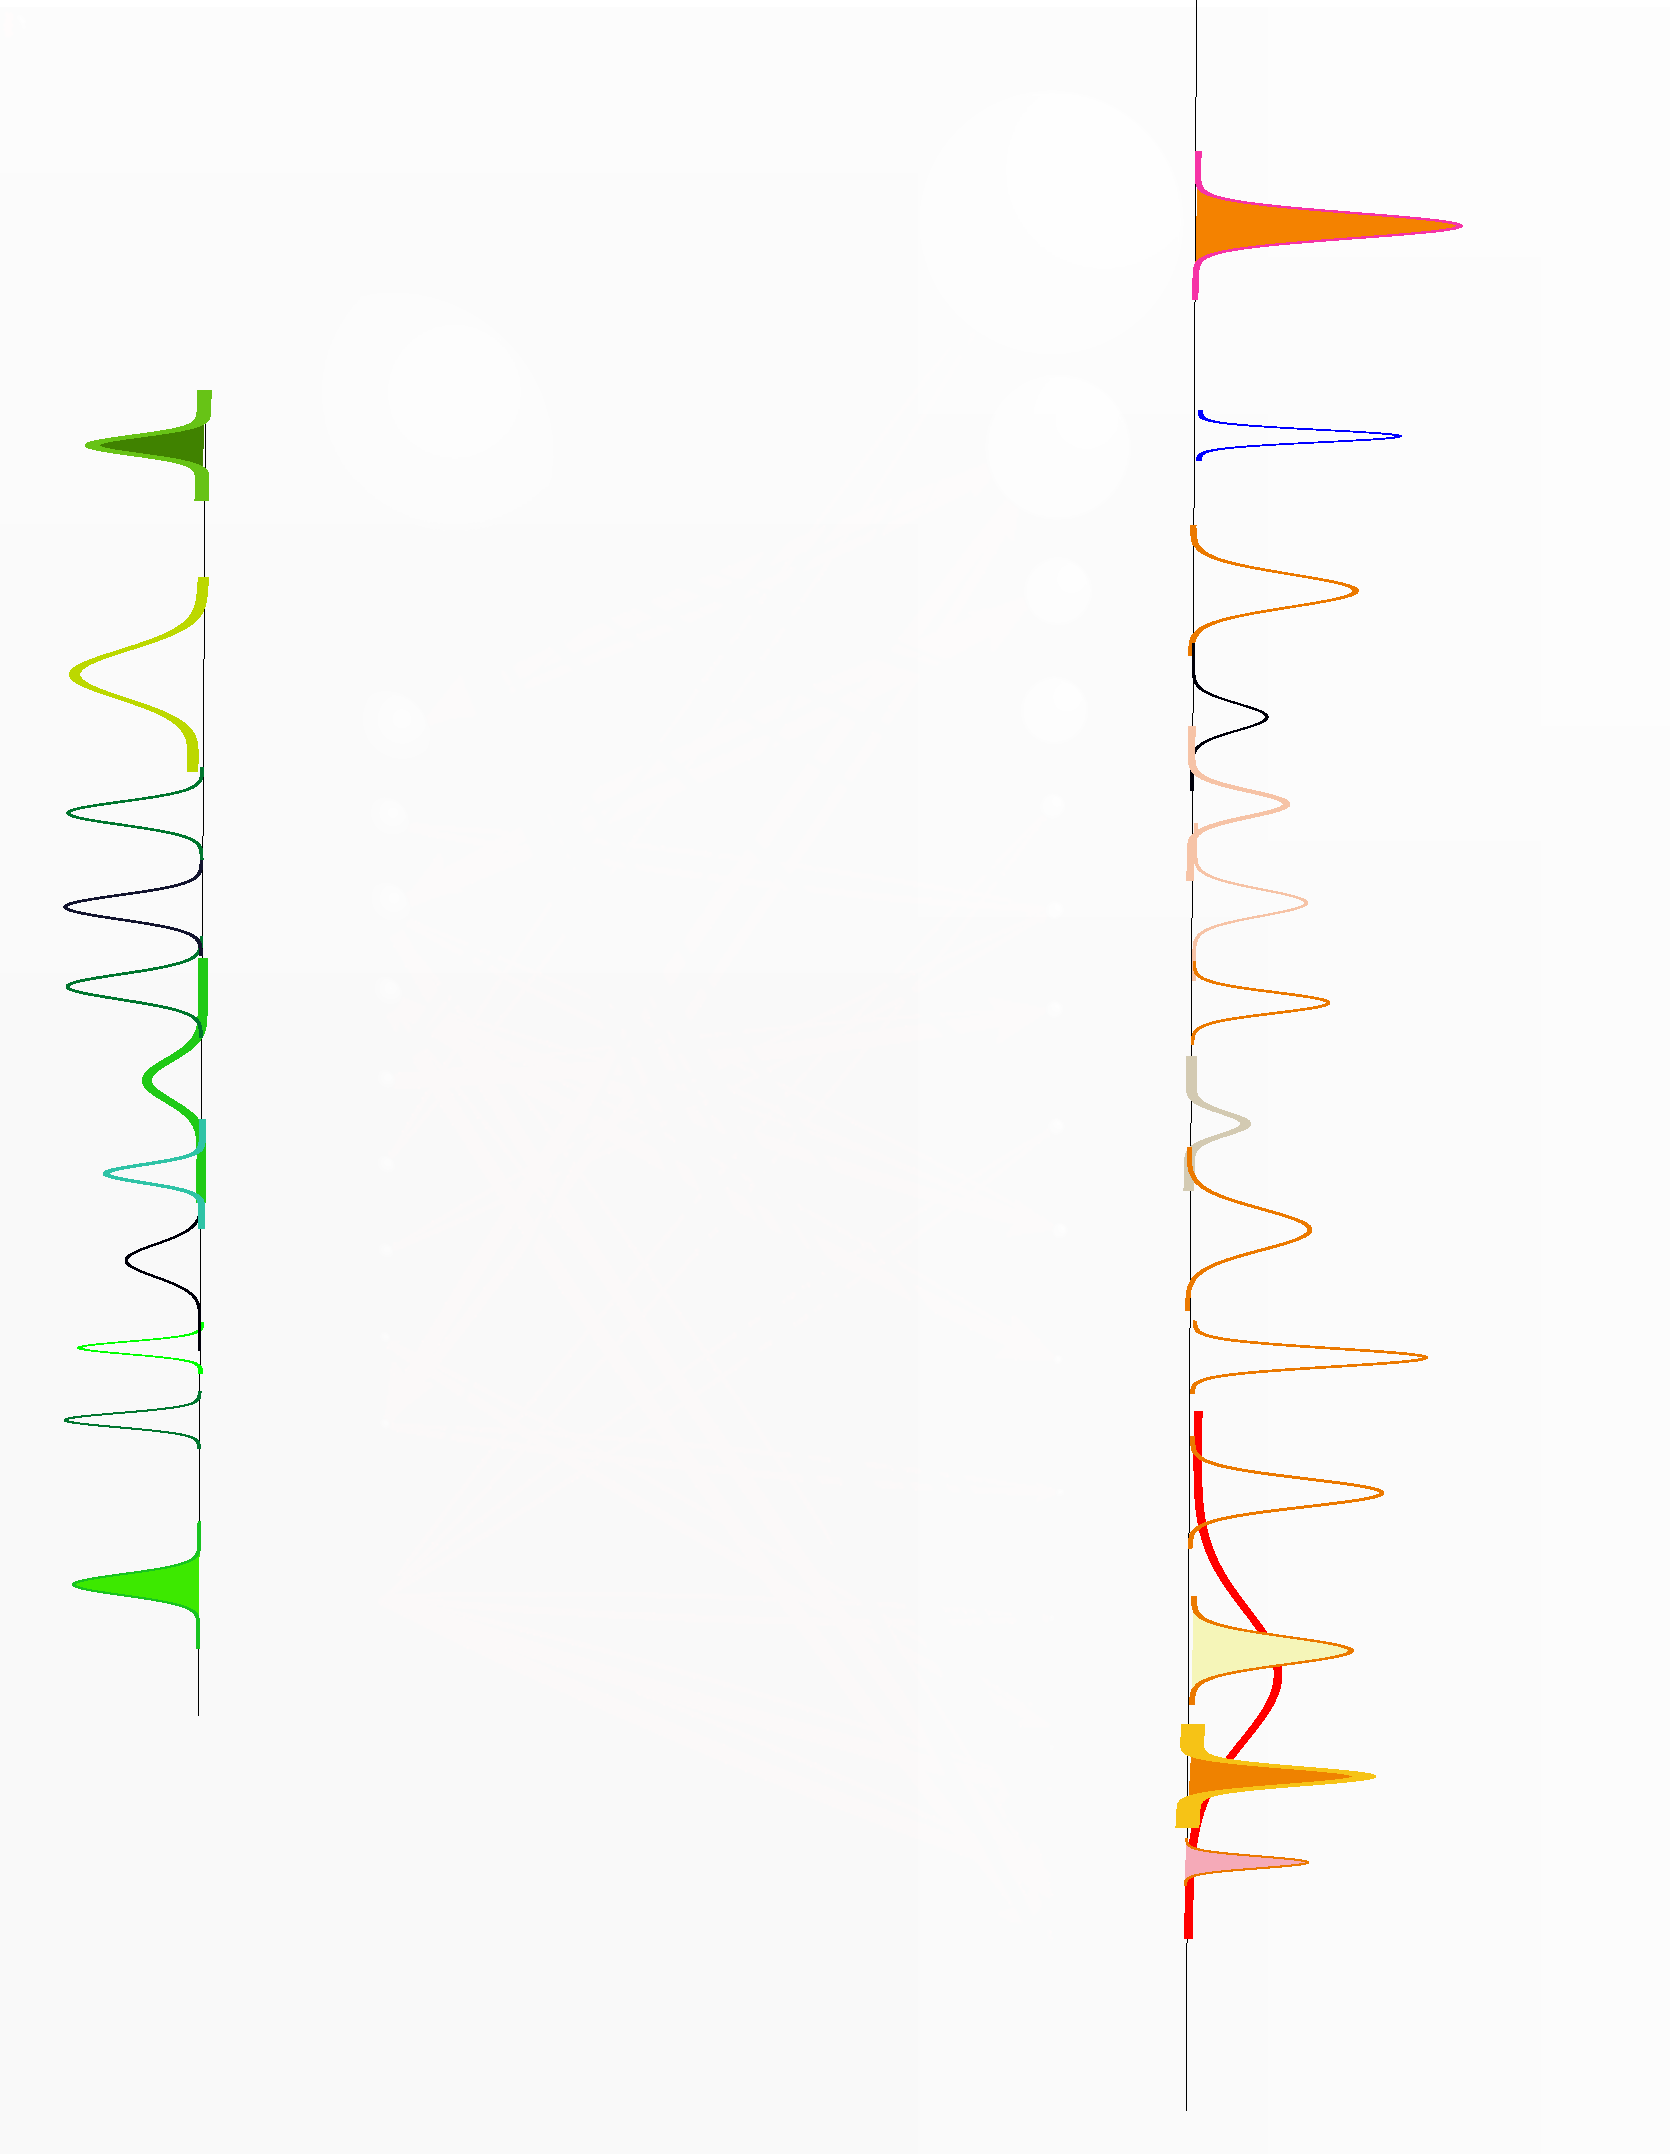
\includegraphics[height=10cm,width=7cm,angle=90]{Slide2.pdf}
\end{beamerboxesrounded}
}

\subsection{Model abundance}
\frame{\frametitle{Modeling eco-evolutionary networks}
\vspace{-0.5 in}
\begin{align} 
 \Delta V_{i} = \textcolor{blue}{r_{i}(t)} V_{i} - c_{i} (V_{i})^{2} - \sum_{j=1}^{N_{E}}  X_{ij} \textcolor{red}{\alpha_{ij}(t)} E_{j} V_{i}\\
 \Delta E_{j} = \textcolor{blue}{r_{j}(t)} E_{j} - c_{j} (E_{j})^{2} - \sum_{j=1}^{N_{V}}  X_{ji} \textcolor{red}{\alpha_{ji}(t)} E_{j} V_{i},
\end{align}
where \textcolor{red}{$\alpha_{ij}(t)$} and \textcolor{blue}{$r_{i}(t)$} are given by
%\vspace{-0.5 in}
 \[
 \boxed{\textcolor{red}{\alpha_{ij}(t) =  \alpha_{ji}(t)} = e^{-{\bf\gamma}(\textcolor{orange}{z_{i}(t)} - \textcolor{violet}{y_{j}(t)})^{2}}; \textcolor{blue}{r_{i}(t)} =  b_{i} - (1 - e^{-{\bf\beta}(\theta_{i}(t) - \textcolor{orange}{z_{i}(t)})^{2}})}
 \]
 and mean trait values are calculated as
 \[
 \boxed{\textcolor{orange}{z_{i(t)}} = z_{i(t-1)} + \phi_{i}(Z_{i}(t-1) - z_{i}(t-1))}
\]
\[
 \boxed{\textcolor{violet}{y_{j(t)}} = y_{j(t-1)} + \phi_{j}(Y_{j}(t-1) - y_{j}(t-1))}
\]
}

\subsection{Mean Abun and traits}
\frame{\frametitle{}
  %\setbeamercolor{uppercol}{fg=black,bg=pink}
  %\setbeamercolor{lowercol}{fg=black,bg=pink}
  \vspace{0.35 in}
%\begin{beamerboxesrounded}[upper=upperco,lower=lowercol,shadow=true]{}
  \hspace{-0.25 in}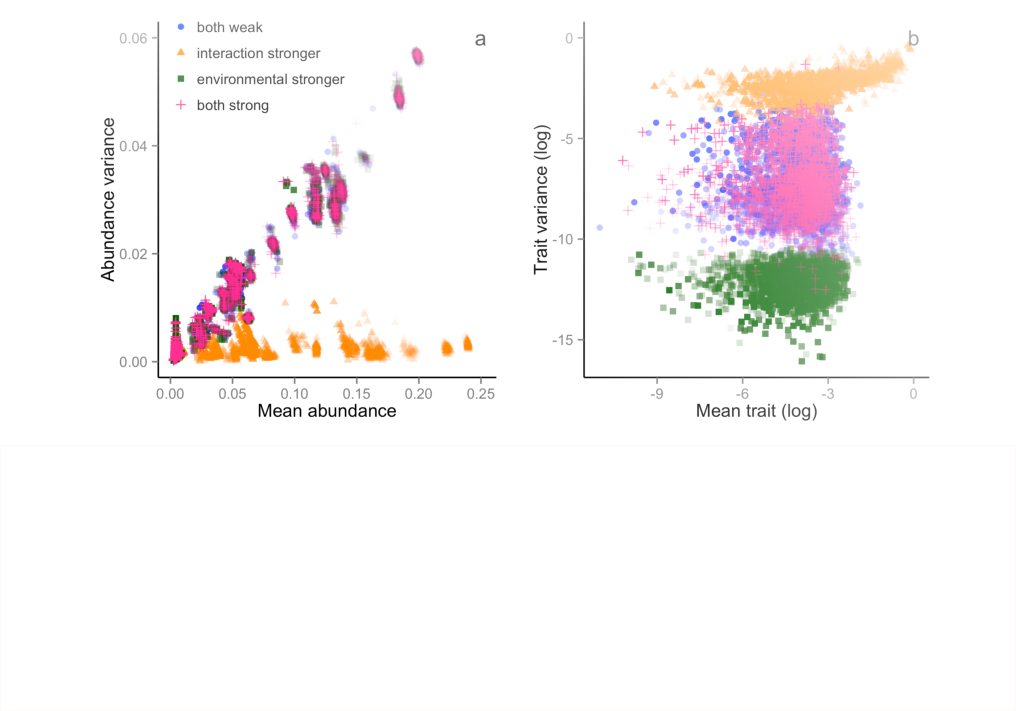
\includegraphics[width=7cm,height=8
  cm]{figure2.pdf}\\
%\end{beamerboxesrounded}
}

\subsection{Fluctuating selection}
\frame{\frametitle{}
\vspace{-0.05 in}
{\tiny The temporal fluctuation in the interaction strength among species pairs, $s_{ij}$, is given by}
 \[
   \boxed{s_{ij}(t) =  X_{ij} \sum_{t=1}^{t=N} |(z_{i(t)} - y_{j(t)}) - (z_{i(t - 1)} - y_{j(t - 1})|,}
 \]
{\tiny The cumulative change in pairwise matching for each victim (exploiter) is} 
 \[
   \boxed{s_{i} = \sum_{j=1}^{N_E} s_{ij},}
 \]
 {\tiny and the mean and variance in cumulative change in pairwise matching in the network is}
 \[
  \boxed{s = \sum_{i=1}^{N_V} \sum_{j=1}^{N_E} s_{ij}/(N_{V} N_{E}); \sigma^2_{s} = (\sum_{i=1}^{N_V} (s_{i} - s)^2 + \sum_{j=1}^{N_E}  (s_{j} - s)^2) /(N_{V} N_{E})}
 \]
}}

\subsection{Fluctuating selection}
\frame{\frametitle{}
\setbeamercolor{uppercol}{fg=black,bg=pink}
\setbeamercolor{lowercol}{fg=black,bg=pink} 
\begin{beamerboxesrounded}[upper=upperco,lower=lowercol,shadow=true]{}
  \hspace{0.25 in}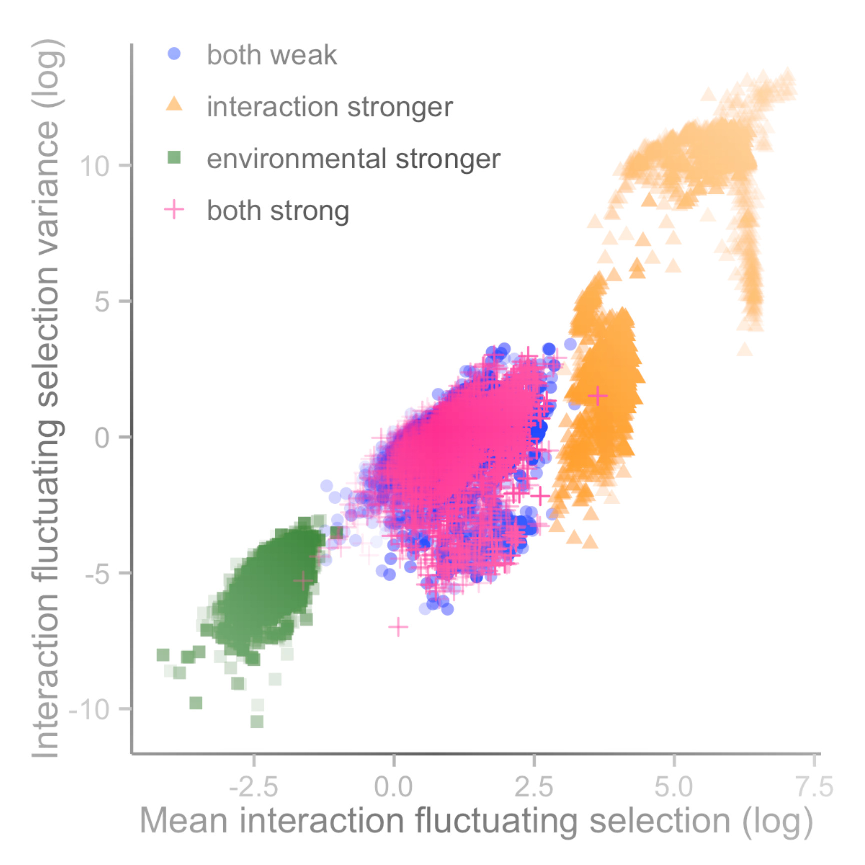
\includegraphics[width=7cm,height=7cm]{figure1.pdf}\\
\end{beamerboxesrounded}
}

\section{Outlook}
\subsection{Outlook}
\frame{\frametitle{Outlook}
\begin{itemize}[<+->]
\item < 1-| alert@1 > \alert{Eco-evolutionary networks} running on interaction trait distributions show many selection regimes, from fluctuating to directional and stabilizing selection.
\item < 2-| alert@2 > \alert{Rapid trait} co-evolution when biotic interactions are stronger than environmental stressors drive higher and less variable abundances.
\item < 3-| alert@3 > Eco-evolutionary networks can be highly persistent despite strong interactions yet environmental stressors and reduction of functional trait variance might rapidly alter population fluctuations and the persistence of these networks.
\end{itemize}
}
    
\subsection{thankyou}
\frame{\frametitle{Merci!}
\begin{itemize}
\item Swiss National Science Foundation 
\item Cecilia S. de Andreazzi, Jordi Bascompte, Miguel A. Fortuna, Paulo Guimaraes, Jan Klecka, Ayana Martins, Gian Marco Palamara, Alex Rozenfeld, Charles N. de Santana, and Ole Seehausen
\end{itemize}
}



\end{document}
